%===============================================================================
% LaTeX sjabloon voor de bachelorproef toegepaste informatica aan HOGENT
% Meer info op https://github.com/HoGentTIN/latex-hogent-report
%===============================================================================

\documentclass[dutch,dit,thesis]{hogentreport}

% TODO:
% - If necessary, replace the option `dit`' with your own department!
%   Valid entries are dbo, dbt, dgz, dit, dlo, dog, dsa, soa
% - If you write your thesis in English (remark: only possible after getting
%   explicit approval!), remove the option "dutch," or replace with "english".

\usepackage{lipsum} % For blind text, can be removed after adding actual content
\usepackage{longtable}

%% Pictures to include in the text can be put in the graphics/ folder
\graphicspath{{graphics/}}

%% For source code highlighting, requires pygments to be installed
%% Compile with the -shell-escape flag!
\usepackage[section]{minted}
%% If you compile with the make_thesis.{bat,sh} script, use the following
%% import instead:
% \usepackage[section,outputdir=../output]{minted}
\usemintedstyle{solarized-light}
\definecolor{bg}{RGB}{253,246,227} %% Set the background color of the codeframe

%% Change this line to edit the line numbering style:
\renewcommand{\theFancyVerbLine}{\ttfamily\scriptsize\arabic{FancyVerbLine}}

%% Macro definition to load external java source files with \javacode{filename}:
\newmintedfile[javacode]{java}{
    bgcolor=bg,
    fontfamily=tt,
    linenos=true,
    numberblanklines=true,
    numbersep=5pt,
    gobble=0,
    framesep=2mm,
    funcnamehighlighting=true,
    tabsize=4,
    obeytabs=false,
    breaklines=true,
    mathescape=false
    samepage=false,
    showspaces=false,
    showtabs =false,
    texcl=false,
}

% Other packages not already included can be imported here

%%---------- Document metadata -------------------------------------------------
% TODO: Replace this with your own information
\author{Tuur Vandamme}
\supervisor{Mevr. L. Vuyge}
\cosupervisor{Mevr. J. Lipkens}
\title{Kan Robotic Process Automation bij klantenservice ingezet worden om een consultant sneller toegang te geven tot nodige informatie?}
\academicyear{\advance\year by -1 \the\year--\advance\year by 1 \the\year}
\examperiod{1}
\degreesought{\IfLanguageName{dutch}{Professionele bachelor in de toegepaste informatica}{Bachelor of applied computer science}}
\partialthesis{false} %% To display 'in partial fulfilment'
\institution{delaware}

%% Add global exceptions to the hyphenation here
\hyphenation{back-slash}

%% The bibliography (style and settings are  found in hogentthesis.cls)
\addbibresource{bachproef.bib}            %% Bibliography file
\addbibresource{../voorstel/voorstel.bib} %% Bibliography research proposal
\defbibheading{bibempty}{}

%% Prevent empty pages for right-handed chapter starts in twoside mode
\renewcommand{\cleardoublepage}{\clearpage}

\renewcommand{\arraystretch}{1.2}

%% Content starts here.
\begin{document}

%---------- Front matter -------------------------------------------------------

\frontmatter

\hypersetup{pageanchor=false} %% Disable page numbering references
%% Render a Dutch outer title page if the main language is English
\IfLanguageName{english}{%
    %% If necessary, information can be changed here
    \degreesought{Professionele Bachelor toegepaste informatica}%
    \begin{otherlanguage}{dutch}%
       \maketitle%
    \end{otherlanguage}%
}{}

%% Generates title page content
\maketitle
\hypersetup{pageanchor=true}

%%=============================================================================
%% Voorwoord
%%=============================================================================

\chapter*{\IfLanguageName{dutch}{Woord vooraf}{Preface}}%
\label{ch:voorwoord}

%% TODO:
%% Het voorwoord is het enige deel van de bachelorproef waar je vanuit je
%% eigen standpunt (``ik-vorm'') mag schrijven. Je kan hier bv. motiveren
%% waarom jij het onderwerp wil bespreken.
%% Vergeet ook niet te bedanken wie je geholpen/gesteund/... heeft

\lipsum[1-2]
%%=============================================================================
%% Samenvatting
%%=============================================================================

% TODO: De "abstract" of samenvatting is een kernachtige (~ 1 blz. voor een
% thesis) synthese van het document.
%
% Een goede abstract biedt een kernachtig antwoord op volgende vragen:
%
% 1. Waarover gaat de bachelorproef?
% 2. Waarom heb je er over geschreven?
% 3. Hoe heb je het onderzoek uitgevoerd?
% 4. Wat waren de resultaten? Wat blijkt uit je onderzoek?
% 5. Wat betekenen je resultaten? Wat is de relevantie voor het werkveld?
%
% Daarom bestaat een abstract uit volgende componenten:
%
% - inleiding + kaderen thema
% - probleemstelling
% - (centrale) onderzoeksvraag
% - onderzoeksdoelstelling
% - methodologie
% - resultaten (beperk tot de belangrijkste, relevant voor de onderzoeksvraag)
% - conclusies, aanbevelingen, beperkingen
%
% LET OP! Een samenvatting is GEEN voorwoord!

%%---------- Nederlandse samenvatting -----------------------------------------
%
% TODO: Als je je bachelorproef in het Engels schrijft, moet je eerst een
% Nederlandse samenvatting invoegen. Haal daarvoor onderstaande code uit
% commentaar.
% Wie zijn bachelorproef in het Nederlands schrijft, kan dit negeren, de inhoud
% wordt niet in het document ingevoegd.

% \IfLanguageName{english}{%
% \selectlanguage{dutch}
% \chapter*{Samenvatting}
% \lipsum[1-4]
% \selectlanguage{english}
% }{}

%%---------- Samenvatting -----------------------------------------------------
% De samenvatting in de hoofdtaal van het document

% Daarom bestaat een abstract uit volgende componenten:
%
% - inleiding + kaderen thema
% - probleemstelling
% - (centrale) onderzoeksvraag
% - onderzoeksdoelstelling
% - methodologie
% - resultaten (beperk tot de belangrijkste, relevant voor de onderzoeksvraag)
% - conclusies, aanbevelingen, beperkingen

\chapter*{\IfLanguageName{dutch}{Samenvatting}{Abstract}}

De werking van een bedrijf bestaat uit honderden processen. Deze kunnen gaan van het aannemen van een nieuwe werknemer, het verkopen van een software licentie tot het dagelijks overzetten van honderd verkooporders van een Excel bestand naar een ERP systeem.
Deze processen zijn zeer gevarieerd, zowel in hun lengte, complexiteit als in de toegevoegde waarde binnen het bedrijf. Het is duidelijk dat het laatstgenoemde proces, het overzetten van de verkooporders, een belangrijke maar vrij repetitieve taak is.
De werknemer die deze taak moet uitvoeren verliest hier dagelijks serieus wat tijd aan, terwijl de meerwaarde voor het bedrijf hier relatief klein is.
En net deze soort repetitieve taken zijn te automatiseren via Robotic Process Automation (RPA). RPA is een recente technologie die een menselijke gebruiker kan nabootsen en deze repetitieve taken feilloos kan uitvoeren via een hardware-toestel van de gebruiker.
Maar is dit wel echt een optie binnen de bedrijfswereld? Hoe werkt deze nieuwe technologie precies en in welke bedrijfstakken kan deze gebruikt worden? Dit zijn allemaal logische vragen die elk bedrijf die denkt om RPA te implementeren zich ook zal stellen.
Deze bachelorproef zal zich richten op het Belgische IT-consultancy bedrijf delaware en hun mogelijkheden om bepaalde processen tijdens hun klantenwerk te automatiseren via RPA.
Concreet betekent dit dat er onderzocht zal worden waar en hoe RPA kan ingezet worden in het dagelijkse werkleven van de consultants.
Om deze vraag te kunnen beantwoorden werd er eerst een grondige literatuurstudie gedaan naar de RPA technologie zelf, het soort processen dat in aanmerking komt voor automatisering en de verschillende verdelers van RPA software.
Hierna werden verschillende interviews afgenomen met consultants van delaware om enerzijds hun interne kennis van RPA te testen en anderzijds processen te vinden die in aanmerking kwamen om geautomatiseerd te worden via RPA.
Met de informatie die uit de literatuurstudie en de interviews kwam werd dan een specifiek proces en een specifieke RPA-verdeler geselecteerd om een Proof of Concept uit te werken.
Wanneer deze Proof of Concept uitgewerkt was, werd deze getest door de consultant die het proces dagelijks moet uitvoeren.
Hieruit kon afgeleid worden dat de automatisering het proces duidelijk sneller uitvoerde dan de consultant zelf, die ook een positieve reactie gaf over het gebruik van de automatisering.
Hieruit kan afgeleid worden dat RPA zeker een grote meerwaarde kan bieden bij klantenwerk. Deze bachelorproef bewijst de voordelen van RPA en toont aan dat bedrijven er baat bij hebben om meer processen te automatiseren via deze techniek.

%---------- Inhoud, lijst figuren, ... -----------------------------------------

\tableofcontents

% In a list of figures, the complete caption will be included. To prevent this,
% ALWAYS add a short description in the caption!
%
%  \caption[short description]{elaborate description}
%
% If you do, only the short description will be used in the list of figures

\listoffigures

% If you included tables and/or source code listings, uncomment the appropriate
% lines.
\listoftables
%\listoflistings

% Als je een lijst van afkortingen of termen wil toevoegen, dan hoort die
% hier thuis. Gebruik bijvoorbeeld de ``glossaries'' package.
% https://www.overleaf.com/learn/latex/Glossaries

%---------- Kern ---------------------------------------------------------------

\mainmatter{}

% De eerste hoofdstukken van een bachelorproef zijn meestal een inleiding op
% het onderwerp, literatuurstudie en verantwoording methodologie.
% Aarzel niet om een meer beschrijvende titel aan deze hoofdstukken te geven of
% om bijvoorbeeld de inleiding en/of stand van zaken over meerdere hoofdstukken
% te verspreiden!

%%=============================================================================
%% Inleiding
%%=============================================================================

\chapter{\IfLanguageName{dutch}{Inleiding}{Introduction}}%
\label{ch:inleiding}

De inleiding moet de lezer net genoeg informatie verschaffen om het onderwerp te begrijpen en in te zien waarom de onderzoeksvraag de moeite waard is om te onderzoeken. In de inleiding ga je literatuurverwijzingen beperken, zodat de tekst vlot leesbaar blijft. Je kan de inleiding verder onderverdelen in secties als dit de tekst verduidelijkt. Zaken die aan bod kunnen komen in de inleiding~\autocite{Pollefliet2011}:

\begin{itemize}
  \item context, achtergrond
  \item afbakenen van het onderwerp
  \item verantwoording van het onderwerp, methodologie
  \item probleemstelling
  \item onderzoeksdoelstelling
  \item onderzoeksvraag
  \item \ldots
\end{itemize}

\section{\IfLanguageName{dutch}{Probleemstelling}{Problem Statement}}%
\label{sec:probleemstelling}

Uit je probleemstelling moet duidelijk zijn dat je onderzoek een meerwaarde heeft voor een concrete doelgroep. De doelgroep moet goed gedefinieerd en afgelijnd zijn. Doelgroepen als ``bedrijven,'' ``KMO's'', systeembeheerders, enz.~zijn nog te vaag. Als je een lijstje kan maken van de personen/organisaties die een meerwaarde zullen vinden in deze bachelorproef (dit is eigenlijk je steekproefkader), dan is dat een indicatie dat de doelgroep goed gedefinieerd is. Dit kan een enkel bedrijf zijn of zelfs één persoon (je co-promotor/opdrachtgever).

\section{\IfLanguageName{dutch}{Onderzoeksvraag}{Research question}}%
\label{sec:onderzoeksvraag}

Wees zo concreet mogelijk bij het formuleren van je onderzoeksvraag. Een onderzoeksvraag is trouwens iets waar nog niemand op dit moment een antwoord heeft (voor zover je kan nagaan). Het opzoeken van bestaande informatie (bv. ``welke tools bestaan er voor deze toepassing?'') is dus geen onderzoeksvraag. Je kan de onderzoeksvraag verder specifiëren in deelvragen. Bv.~als je onderzoek gaat over performantiemetingen, dan 

\section{\IfLanguageName{dutch}{Onderzoeksdoelstelling}{Research objective}}%
\label{sec:onderzoeksdoelstelling}

Wat is het beoogde resultaat van je bachelorproef? Wat zijn de criteria voor succes? Beschrijf die zo concreet mogelijk. Gaat het bv.\ om een proof-of-concept, een prototype, een verslag met aanbevelingen, een vergelijkende studie, enz.

\section{\IfLanguageName{dutch}{Opzet van deze bachelorproef}{Structure of this bachelor thesis}}%
\label{sec:opzet-bachelorproef}

% Het is gebruikelijk aan het einde van de inleiding een overzicht te
% geven van de opbouw van de rest van de tekst. Deze sectie bevat al een aanzet
% die je kan aanvullen/aanpassen in functie van je eigen tekst.

De rest van deze bachelorproef is als volgt opgebouwd:

In Hoofdstuk~\ref{ch:stand-van-zaken} wordt een overzicht gegeven van de stand van zaken binnen het onderzoeksdomein, op basis van een literatuurstudie.

In Hoofdstuk~\ref{ch:methodologie} wordt de methodologie toegelicht en worden de gebruikte onderzoekstechnieken besproken om een antwoord te kunnen formuleren op de onderzoeksvragen.

% TODO: Vul hier aan voor je eigen hoofstukken, één of twee zinnen per hoofdstuk

In Hoofdstuk~\ref{ch:conclusie}, tenslotte, wordt de conclusie gegeven en een antwoord geformuleerd op de onderzoeksvragen. Daarbij wordt ook een aanzet gegeven voor toekomstig onderzoek binnen dit domein.
\chapter{\IfLanguageName{dutch}{Stand van zaken}{State of the art}}%
\label{ch:stand-van-zaken}

Robotic Process Automation (RPA) is de laatste jaren opgekomen als een van de belangrijkste nieuwe technologiën op het vlak van automatiseringen en digitale transformatie. RPA maakt gebruik van software 'robots' om repetitieve, tijdrovende en foutgevoelige taken te automatiseren. Hierdoor kunnen bedrijven hun processen efficiënter maken, kosten verlagen en productiviteit verhogen. RPA zorgt er ook voor dat werknemers zich niet meer hoeven te focussen op deze taken, waardoor ze zich, volgens het onderzoek van \textcite{ZalewskaTurzynska2022} meer kunnen focussen op het creëren van meerwaarde en zich kunnen focussen op inovatievere taken. Omdat RPA meer blijkt te zijn dan een nieuw buzzwoord en hierdoor in verschillende sectoren aan populariteit blijft winnen, is het een onderwerp waar er recent veel belangstelling aan wordt gehecht.

% Tip: Begin elk hoofdstuk met een paragraaf inleiding die beschrijft hoe
% dit hoofdstuk past binnen het geheel van de bachelorproef. Geef in het
% bijzonder aan wat de link is met het vorige en volgende hoofdstuk.

% Pas na deze inleidende paragraaf komt de eerste sectiehoofding. 

% \section{Robotic Process Automation in 2024}

Het onderwerp van deze bachelorproef is het analyseren van Robotic Process Automation, de verschillende verkopers van deze software en dit toepassen op een process voor het consultancy bedrijf delaware. In een eerste deel kijken we hoe RPA precies ontstaan is, wat het inhoud en welke processen in aanmerking komen op geautomatiseerd te worden. In een tweede deel onderzoeken we de voor- en nadelen van de verschillende RPA-software verdelers.

\section{Robotic Process Automation}

Robotic Process Automation is nog steeds een relatief nieuwe technologie. Het verschilt van andere automatiserings-software in de manier waarop het interaggeert met de applicaties. Waar klassieke automatiseringstools 'inside-out' werken en dus in de applicatie-software zelf worden ingewerkt, werkt RPA op een 'outside-in' manier. Dit wil zeggen dat een RPA-automatisering werkt op de presentatielaag van een applicatie. Hier voert de automatisering taken uit zoals een eindgebruiker deze zou uitvoeren, maar volgens \textcite{Bras2023} met een hogere snelheid en precisie. Doordat RPA op deze manier werkt is er een minimale aanpassing nodig om een RPA-automatisering binnen een systeem te implementeren \autocite{Ivancic2019}.
Deze manier van interageren met de presentatielaag wordt bereikt door middel van agents die software 'robots' kunnen aansturen. Een agent is een hardware-systeem (desktop, laptop, virtual machine, etc.) waarop de RPA-software is geïnstalleerd. Wanneer de RPA-software deze agent in werking zet, zal deze agent een software 'robot' starten die vervolgens het systeem overneemt en de automatisering uitvoert. Deze automatisering is dan in staat om een eindgebruiker van het systeem na te bootsen en via toetsaanslagen en muisbewegingen verschillende taken uit te voeren. Wanneer een deze robot de automatisering heeft uitgevoerd, gaat hij terug in een slaapstand waardoor de gebruiker weer volledige controle krijgt over het hardware-systeem en wacht de agent op een nieuwe taak.
Zoals besproken door \textcite{Ivancic2019} hebben we bij RPA 2 verschillende soorten robots, attended en unatteded robots. Attended bots zijn software-robots die automatiseringen uitvoeren samen met een gebruiker. De robot voert bepaalde taken uit, maar geeft informatie terug aan een gebruiker die deze output controleerd, kan gebruiken in andere processen, etc. De unattended robots daarentegen, werken volledig autonoom en kunnen hun taak uitvoeren zonder tussenkomst van een gebruiker. Dit zijn vaak complexere taken met een grote hoeveelheid data die zeer repetitief verwerkt moet worden en waar de gebruiker geen meerwaarde van ondervindt om deze te controleren.

\section{Het ontstaan van Robotic Process Automation}

\subsection{De begindagen van automatisering}

Het idee om repetitieve, handmatige taken te automatiseren is niet nieuw.
Automatisering maakt al decennia lang deel uit van de industrie. Sinds de industriële revolutie zijn vele taken die vroeger handmatig werden uitgevoerd, vervangen door machines en robots. Denk hierbij bijvoorbeeld aan de lopende band-productie. Het toepassen van automatiseringstechnieken in bedrijfsprocessen en administratie is echter een recentere ontwikkeling, die we te danken hebben aan deze eerste successen binnen de industrie.

\subsection{Het begin van Robotic Process Automation}

Het succes van automatiseringen in de industrie heeft ervoor gezorgd dat bedrijven ook in andere bedrijfsprocessen onderzoek zijn gestart om deze concepten toe te kunnen passen. Eind jaren 90 werden de eerste software-robots ontwikkeld die routinetaken in de productieomgeving konden automatiseren. Deze software-robots waren echter nog niet van de omvang die we vandaag kennen, maar lijken volgens \textcite{ZalewskaTurzynska2022} meer op de huidige 'macros' die we kennen vanuit Microsoft Excel. Deze software-robots konden repetitieve taken uitvoeren in 1 applicatie, maar waren niet in staat om verschillende applicaties aan te spreken. Maar zelfs bij het automatiseren van deze eenvoudige, repetitieve basistaken, zoals gegevensinvoer en basisprocesbeheer, werd RPA toch al snel gezien als een waardevol hulpmiddel om de efficiëntie te verhogen en kosten te verlagen.

Sinds midden 2000 werd deze automatisering door verschillende bedrijven uitgebreid naar de wat we nu kennen als het begin van de Robotic Process Automation. Hierdoor werd het mogelijk om automatiseringen handelingen te laten uitvoeren in verschillende applicaties \autocite{Fluss2020}, waardoor de mogelijkheden van deze automatiseringen snel de lucht in gingen.

Hierdoor begonnen bedrijven de potentie van RPA te zien, maar het is pas later, rond 2010, dat RPA echt aan populariteit begon te winnen.

\subsection{Robotic Process Automation als mainstream technologie}

Zoals hierboven vermeld nam in 2010 het gebruik van RPA-technologiën aanzienlijk toe. Grote bedrijven, die werken met een complex IT-landschap die over de jaren heen bleef groeien, werden zich bewust van de potentiële kostenbesparingen en verbeterde efficiëntie die deze nieuwe technologie bood. De ontwikkeling van cloudgebaseerde RPA-software maakte de technologie ook veel toegankelijker aangezien er nu geen grote investeringen in een uitgebreide IT-infrastructuur meer nodig was.

Sinds 2010 is de RPA-markt elk jaar blijven toenemen. Volgens \textcite{Jiles2020} beginnen bedrijven vaak met RPA in de financiële afdeling, maar dit wordt meestal snel uitgebreid naar de verschillende bedrijfstakken. Door de vele interesse in de RPA technologie zijn de verschillende verdelers van deze software ook gegroeid, waardoor hun software steeds meer functionaliteiten aanbiedt en de mogelijkheden van RPA steeds groter worden. Ook de opkomst van nieuwe technologiën, zoals artificiële intelligentie (AI) en machinaal leren (ML) zorgen ervoor dat RPA steeds meer mogelijkheden biedt.

\subsection{De toekomst van Robotic Process Automation}

De oorsprong van RPA gaat terug tot eind jaren negentig, toen de eerste software-automatiseringen to stand kwamen. In de loop der tijden is RPA geevolueerd van een eenvoudige manier van automatiseren tot een volwaardige, mainstream en multifunctionele technologie waarmee bedrijven verschillende bedrijfprocessen kunnen automatiseren.

De voorbije jaren is de interesse in RPA duidelijk nog steeds toegenomen, aangezien RPA volgens \textcite{Laxmikant2023} een van de top 10 technologische trends is voor de komende 5 tot 10 jaar. Nieuwe technologiën zoals AI en ML, die steeds meer worden toegepast binnen de RPA-software, zorgen opnieuw voor extra mogelijheden binnen de RPA-technologie. Deze mogelijkheden zullen er voor zorgen dat RPA nog complexere taken zal kunnen uitvoeren, waardoor de mogelijkheden voor RPA nog zullen toenemen.

De toekomst voor RPA ziet er veelbelovend uit, aangezien het gezien wordt als een van de tien technologiën die we in de gaten moeten houden in de komende jaren.

\section{Onderliggende technologiën}

Zoals we hierboven hebben besproken is RPA vrij recent ontstaan. Automatiseringen zelf bestaan al een heel stuk langer. De technologiën die RPA mogelijk maken zijn dus ook niet nieuw meer. Hieronder bespreken we de belangrijkste bouwblokken die RPA mogelijk maken.

\subsection{Presentatielaag (GUI)}

We hebben besproken dat RPA op een 'outside-in' manier werkt. RPA gebruikt de presentatielaag zoals een normale gebruiker deze zou gebruiken. Onder presentatielaag verstaan we hier de laag van een applicatie die een gebruiker kan zien, en waarmee hij kan interageren via toetsaanslagen en muisbewegingen \autocite{ZalewskaTurzynska2022}.

\subsection{Screen Scraping}

Screen scraping is een techniek die werd gebruikt om de presentatielaag van een applicatie uit te lezen, waardoor deze gegevens gebruikt kunnen worden in een andere applicatie \autocite{Spencer2018}. Deze techniek wordt ook door RPA gebruikt, maar op een gesofisticeerdere manier. Oudere screen scraping software was niet in staat om elementen van een applicatie te herkennen, maar gebruikte vooral de relatieve positie van elementen om deze te kunnen gebruiken. Dit gaf natuurlijk problemen wanneer de presentatielaag aangepast werd, aangezien de relatieve positie van de elementen dan ook aangepast werd. Hierdoor werd het dus moeilijk om robuuste automatiseringen te maken die niet snel zouden falen. \textcite{Asquith2019} spreekt over de identificatie van de elementen van een bepaalde pagina, waardoor RPA-software weet waarmee het moet interageren, en hierdoor dus minder afhankelijk is van de applicatie-layout en dus foutbestendiger kan werken.

\subsection{Optical Character Recognition (OCR)}

Bij sommige automatiseringen is het ook nodig om verschillende documenten te kunnen uitlezen. OCR is een technologie die het mogelijk maakt om tekst uit verschillende documenten te kunnen lezen. Denk hierbij aan e-mails van klanten, facturen, etc. Dit maakt het mogelijk voor RPA-automatiseringen om ook deze gegevens uit te lezen en te kunnen gebruiken in andere applicaties \autocite{ZalewskaTurzynska2022}.

\subsection{Application Programming Interface (API)}

Een extra voordeel van RPA-software is het feit dat het ook gebruik kan maken van API-calls om data te verzamelen. Dit vergroot de mogelijkheden om nog meer systemen samen te laten werken, op een snellere en robuustere manier. Vooral bij het automatiseren van processen die veel data nodig hebben om taken uit te voeren, is deze extra mogelijkheid volgens \textcite{Hofmann2020} een groot pluspunt in vergelijking met de normale, menselijke gebruikers.

\subsection{Data Extraction}

Hierboven hebben we al gesproken over data uit API-calls, maar RPA-software kan ook moeiteloos data uit andere bronnen halen, zoals Microsoft Excel, PDF, e-mails, etc. \autocite{Andrade2022} Opnieuw is dit een voordeel ten opzichte van menselijke gebruikers, aangezien deze data vaak in grote pakken beschikbaar is en moeilijker leesbaar is voor menselijke gebruikers.

\subsection{Artificiële Intelligentie (AI) en Machinaal Leren (ML)}

In het deel 'Robotic Process Automation als mainstream technologie' hebben we al eens AI en ML vermeld als technologiën die RPA gunstig kunnen beïnvloeden. Deze technologiën worden vaker en vaker ingezet bij RPA-software, waardoor de robots complexere taken kunnen behandelen, die meer intelligentie zullen vereisen. Denk hierbij aan het herkennen van afbeeldingen, teksten en e-mails begrijpen, etc. RPA-software zal ook kunnen leren van zijn eigen fouten, waardoor het mogelijk zal zijn om robuustere automatiseringen te maken, die zichzelf constant zelf kunnen verbeteren \autocite{Taulli2020}.

\section{Robotic Process Automation in de bedrijfswereld}

Als we de voordelen van RPA bekijken, is het niet verbazend dat het de laatste jaren zo aan populariteit heeft gewonnen, vooral in de bedrijfswereld. RPA biedt bedrijven de kans om verschillende processen te automatiseren, waardoor de efficiëntie van deze bedrijven de hoogte kan ingaan. Onderzoek leert ons natuurlijk wel dat niet elk process enven geschikt is om geautomatiseerd te worden, en dat de juiste keuze van processen belangrijk is voor het succes van de implementatie van een RPA-automatisering binnen een bepaald bedrijf. Hieronder bespreken we RPA binnen een bedrijfsomgeving.

\subsection{Stroomlijnen van bedrijfsprocessen}

Bedrijven zijn constant op zoek naar mogelijkheden om hun bedrijfprocessen te verbeteren. Hierbij kunnen verhoogde snelheid, verhoogde efficiëntie en besparingen de drijfveren zijn \autocite{Axmann2022}. Zoals hierboven beschreven, lijkt RPA een ideale oplossing te zijn om deze doelen te bereiken. Elke bedrijf heeft verschillende repetitieve processen die gebasseerd zijn op vaste regels, die werken met een groot volume aan data en die zeer foutgevoelig zijn. Dit zijn nu net de processen die ideaal zijn om geautomatiseerd te worden. Een extra voordeel hiervan is het feit dat de werknemer zich kan bezighouden met taken die meer menselijk inzicht vragen, en dus van grotere waarde zijn voor het bedrijf. Hierdoor stijgt niet alleen de toegevoegde waarde van deze werknemer, wat dan op zich weer zorgt voor een hogere productiviteit.

\subsection{Kostenbesparing}

RPA is natuurlijk niet de enige automatiseringstool op de markt. Een ander pluspunt waardoor bedrijven vaak in de richting van RPA kijken is volgens \textcite{Fernandez2021} de relatief lage kost. Aangezien RPA werkt op de presentatielaag (outside-in) van een applicatie, hoeft deze applicatie zelf niet of amper aangepast worden, waardoor de downtime van een systeem minimaal is en de RPA-automatisering snel kan worden geïmplementeerd en in gebruik worden genomen \autocite{Asquith2019}. Dit is een groot voordeel ten opzichte van de klassiekere automatiseringsmogelijkheden, die vaak grotere investeringen vragen en een hogere implementatieduur hebben. Hierdoor heeft RPA een relatief korte terugverdientijd (ROI), wat voor bedrijven natuurlijk een groot pluspunt is.
Door deze relatief lage kost is RPA ook niet alleen beschikbaar voor de grote bedrijven en marktleiders, maar zien we dat middelgrote en kleine bedrijven ook steeds meer interesse tonen voor deze technologie.

\section{Verloop van een RPA-project}

Hierboven is al besproken dat RPA met relatief weinig bronnen een hoge ROI kan opleveren.
Maar daarvoor moet RPA natuurlijk wel op de correcte processen worden toegepast.
Een bedrijf bevat duizenden processen in zijn dagelijkse werking, dus in deze paragrafen bespreken we welke stappen we volgens \textcite{El-Gharib2023} moeten ondernemen om een RPA-project succesvol te implementeren.

\subsection{Analyse en proces-evalutaie}

De eerste stap binnen het implementatie-process van RPA is het analyseren van de verschillende processen binnen een bedrijf die in aanmerking komen om via RPA geautomatiseerd te worden \autocite{vanDerAalst2018}. Hierbij kijken we naar de frequentie van het process, de complexiteit en of de verschillende stappen binnen het process voldoende gestandardiseerd zijn. Wanneer deze factoren tegen de verschillende processen getoetst zijn, kunnen we per process inschatten hoeveel baat we erbij zouden hebben om deze via RPA te automatiseren, en een ruwe schatting maken van onze ROI. Dit doen we door van de verschillende processen alle stappen grondig te analyseren, kijken waar er verbeteringen kunnen optreden in het process en deze in een flow te gieten. Deze flow kunnen we dan analyseren en gebruiken voor de volgende stappen binnen het project.
Na de evaluatie van het process is het natuurlijk ook belangrijk om te kijken welke RPA-software het best past bij onze automatisering, en bij bedrijven is het vaak ook belangrijk om te bekijken welke middelen ze in huis hebben. Hierbij kijken we naar licenties, kennis binnen het bedrijf, etc.

\subsection{Planning en design}

Wanneer een process geselecteerd en ge-analyseerd is voor automatisering, kunnen we beginnen aan de planning en het ontwerp van de automatisering \autocite{Fernandez2021}. Vanuit de analyse-stap komt een flow-diagram die het beginpunt kan zijn van het design van de RPA robot. Hierbij wordt gekeken naar de verschillende stappen binnen deze flow en hoe deze best geautomatiseerd kunnen worden binnen de verschillende mogelijkheden van RPA. Wanneer er voor elke stap een oplossing gevonden is, kunnen we een compleet ontwerp maken van de RPA-flow.

\subsection{Ontwikkeling}

In de vorige stap is er een volledig design gemaakt voor de RPA-automatisering. Deze kan nu door de ontwikkelaar gebruikt worden om de RPA robot te ontwikkelen binnen de gekozen RPA-software. Het is belangrijk dat de ontwikkelaar zich bewust is van het process die hij aan het automatiseren is, en niet te ver afdwaalt van de gecreëerde workflow.

\subsection{Testen en validatie}

Wanneer de automatisering ontwikkeld is, is het belangrijk deze voldoende te testen op zowel correctheid als robuustheid \autocite{Liu2023}. Hierbij is het belangrijk dat zowel de 'happy flow' als de 'exception flows' getest worden. Bij de happy flow is het belangrijk te kijken of de stappen die de automatisering moet uitvoeren correct gebeurd zijn, en bij de exception flow is het belangrijk te kijken of de automatisering hier correct op reageert en de juiste informatie geeft aan de gerbuiker. Ook is het belangrijk dat de automatisering in de exception flow geen verkeerde informatie in een systeem heeft binnengebracht.
In een latere fase van het testen is het mogelijk de RPA-robot in te zetten bij een kleine groep gebruikers of een deel van de uit te voeren processen om te kijken hoe het werkt in de praktijk. Hierna kan bij de gebruikers feedback gevraagd worden, of kunnen de systemen gecontroleerd worden op correcte data.

\subsection{Inzet, onderhoud en monitoring}

Wanneer de RPA-automatisering voldoende getest is kan deze ingezet worden in de volledige praktijk. \textcite{Lievanomartinez2022} beschrijft dat het hierbij natuurlijk belangrijk is dat de gebruikers genoeg opgeleid zijn om te weten hoe de RPA robot werkt, hoe ze hem kunnen gebruiken, welke taken deze overneemt en de robot de nodige middelen heeft om de vooropgestelde taken uit te voeren. Volgens \textcite{vanDerAalst2018} is het natuurlijk ook belangrijk om de RPA-robot te blijven onderhouden, en wanneer er aan de onderliggende systemen aanpassingen worden aangebracht, deze ook opnieuw te controleren op een correcte werking om desastreuze gevolgen te vermijden.
Maar zelfs wanneer er geen aanpassingen aan het systeem zijn gemaakt, is het belangrijk om de verschillende RPA robots te blijven monitoren. Hierdoor kan de performantie van de robots gecontrolleerd worden, en in een volgende stap opnieuw verbeterd worden.

\section{Verschillende verdelers van Robotic Process Automation software}

RPA is een relatief nieuwe, inovatieve technologie. Hierdoor zijn er veel bedrijven die hun eigen RPA-software aanbieden, waardoor het belangrijk is om de verschillende verdelers met elkaar te vergelijken. \textcite{Carter2023} bespreekt het Gartner RPA Magic Quadrant, en welke bedrijven we moeten zien als marktleiders, visionairs, challengers en niche spelers. Hieronder bespreken we de marktleiders, maar ook een belangrijke visionair-optie die voor delaware een grote meerwaarde kan betekenen.

\subsection{UIPath}

UIPath is Roemeens bedrijf, opgericht in 2005. Het is de marktleider van 2023, waar het de trend van 2022 mee verderzet. Het richt zich vooral op end-to-end processen. Ook is het een van de oplossingen die het verste staat in het integreren van AI binnen hun gebied \autocite{GartnerUIPath2023}.

\subsubsection{Voordelen van UIPath}

\begin{itemize}
    \item UIPath is een van de oudste en een van de meest geavanceerde RPA oplossingen op de markt.
    \item UIPath heeft verschillende AI toepassingen geïntegreerd binnen hun volledige platform \autocite{Liliana2022}.
    \item UIPath heeft verschillende tools beschikbaar die het vinden van automatiseerbare processen binnen een bedrijf makkelijker maken.
    \item UIPath heeft meerdere out-of-the-box automatiseringen die direct ingezet en gebruikt kunnen worden binnen een bedrijf.
\end{itemize}


\subsection{Blueprism}

Blue Prism is een Brits bedrijf, opgericht in 2001. Het behoort tot de marktleiders van 2023. Blue Prism richt zich vooral op grotere bedrijven. Voor deze bedrijven heeft het ook verschillende connectoren gecreëerd voor veelgebruikte applicaties binnen bedrijven \autocite{GartnerBluePrism2023}. Ook biedt Blue Prism gebundelde services aan voor deze bedrijven, met meerdere robot licenties, een dashboard, etc. Blue Prism richt zich vooral op unattended end-to-end processen \autocite{Laxmikant2023}.

\subsubsection{Voordelen van Blueprism}

\begin{itemize}
    \item Goed geintegreerde AI en ML toepassingen binnen hun product.
    \item Makkelijk te schalen, wat belangrijk is voor grotere bedrijven.
    \item Toepassingen voor het volledige process van RPA-implementatie, van het zoeken naar processen tot het in gebruik nemen van de automatiseringen.
    \item Vergevorderede Email AI.
\end{itemize}

\subsection{Automation 360}

Automation 360 is een product van het Amerikaans bedrijf Automation Anywhere, opgericht in 2003. Het behoort tot de marktleiders van 2023. Automation 360 richt zich vooral op attended bots. Het werkt via een cloud-platform, waardoor het relatief goedkoop en makkelijk schaalbaar is \autocite{GartnerAutomationAnywhere2023}.

\subsubsection{Voordelen van Automation 360}

\begin{itemize}
    \item Focus op attended robots, die gebruikers helpen met hun dagelijkse taken.
    \item Via hun Process Discovery tool kunnen de processen die het meest baat zullen hebben van automatiseringen ontdekt worden.
    \item Zowel geschikt voor kleine als middelgrote bedrijven.
    \item Volledig cloud gericht.
\end{itemize}

\subsection{Power Automate}

Power Automate is de RPA oplossing van Microsoft. Het behoort ook tot de marktleiders van 2023. Het heeft verschillende connectoren naar verschillende Microsoft producten, wat het aantrekkelijk maakt voor bedrijven die dit ecosysteem gebruiken. Het richt zich zowel op attended als unattended bots \autocite{GartnerMicrosoftPA2023}.

\subsubsection{Voordelen van Power Automate}

\begin{itemize}
    \item Makkelijke connectoren met verschillende Microsoft producten zoals Azure, Power BI, etc.
    \item Een groot aantal out-of-the-box automatiseringen en connectoren.
    \item Goede integratie van API-mogelijkheden.
    \item AI mogelijkheden binnen zowel de creatie als het gebruik van de RPA.
\end{itemize}

\subsection{SAP Build Process Automation}

SAP Build Process Automation is de RPA oplossing van SAP. Het behoort tot de visionairs van 2023. Het werkt makkelijk binnen het SAP ecosysteem, maar is zeker niet beperkt tot deze applicaties. Het richt zich zowel op attended als unattended bots \autocite{GartnerSAPBPA2023}.

\subsubsection{Voordelen van SAP Build Process Automation}

\begin{itemize}
    \item Makkelijke integratie binnen een bestaand SAP Ecosysteem.
    \item Vlotte process analyse via SAP Signavio.
    \item Relatief goedkoop wanneer een bedijf binnen het SAP Ecosysteem werkt.
    \item Goede AI en workflow mogelijkheden.
\end{itemize}
%%=============================================================================
%% Methodologie
%%=============================================================================

\chapter{\IfLanguageName{dutch}{Methodologie}{Methodology}}%
\label{ch:methodologie}

Zoals uit de Hoofdstuk~\ref{ch:stand-van-zaken} is gebleken, is een correct proces kiezen en deze automatiseren niet altijd even eenvoudig. Daarom is het onderzoek binnen deze bachelorproef opgedeeld in 4 grote fases, die hieronder kort besproken worden.

\section{Literatuurstudie}
\label{sec:literatuurstudie}

De eerste fase van het onderzoek is de literatuurstudie. Hierin werd RPA in zijn gehele onderzocht. Er werd zowel gekeken naar het onstaan van RPA, de verschillende technologieën die RPA mogelijk maken en hoe RPA binnen een bedrijfscontext gebruikt kan worden.
Tenslotte werden de verschillende RPA-verdelers besproken.

\section{Interviews met consultants}
\label{sec:interviews-consultants}

Voor de tweede fase van het onderzoek werden 4 verschillende consultants binnen delaware ondervraagd. Met de kennis die in de eerste fase vergaard werd, werden de consultants gericht bevraagd over hun visie op en ervaring met RPA, zowel persoonlijk als binnen delaware. Uit deze interviews werden ook verschillende processen uit hun dagelijkse werkdag gehaald die later in het onderzoek vergeleken werden om zo tot een geschikt proces te komen voor de volgende fase binnen dit onderzoek.

\section{Proof of Concept}
\label{sec:proof-of-concept}

In de derde fase werd, met de kennis uit de vorige twee fases, een Proof of Concept uitgewerkt. Deze fase kan onderverdeeld worden in 3 sub-fases. Deze worden hieronder besproken.

\subsection{Keuze van het proces}
\label{subsec:keuze-proces}

Uit de tweede fase van het onderzoek kwamen verschillende processen die de consultants opgegeven hebben als processen die in aanmerking komen om geautomatiseerd te worden via RPA. Deze processen werden met elkaar vergeleken op verschillende criteria, waar ze per criteria een score op 3 kregen. Deze scores werden dan opgeteld en vergeleken, om zo het proces te kiezen wat volgens deze criteria het best geschikt is om uit te werken als een RPA-automatisering.

\subsection{Keuze van de RPA-software}
\label{subsec:keuze-software}

In de eerste fase van het onderzoek werden verschillende RPA-verdelers onderzocht en vergeleken. In de tweede fase werd dan gekeken naar de verschillende RPA-software waar delaware specifiek al ervaring mee had en hoe gekend deze waren bij de werknemers.
Met deze kennis en de kennis van het gekozen proces werd dan bekeken welke tool het best bij de Proof of Concept past.

\subsection{Uitwerking Proof of Concept}
\label{subsec:uitwerking-proof-of-concept}

Nu het proces en de RPA-software gekend waren, werd de Proof of Concept in de praktijk uitgewerkt. Hiervoor werden de verschilende stappen die in Hoofdstuk~\ref{ch:stand-van-zaken} besproken werden gevolgd.
De gecreëerde automatisering werd binnen deze fase, samen met een consultant, vergeleken met de huidige manier van werken. Hieruit werd dan geconcludeerd of de automatisering wel degelijk een meerwaarde biedt voor de consultant.

\section{Conclusie}
\label{sec:conclusie}

In deze laatste fase werd de conclusie getrokken uit de bevindingen uit de vorige fases. Vanuit deze conclusies werden de onderzoeksvraag en de deelvragen beantwoord. Hierna werd ook de toekomst van RPA binnen delaware besproken.
\chapter{\IfLanguageName{dutch}{Interviews met consultants}{Interviews with consultants}}%
\label{ch:interviews}

Het is belangrijk om te weten hoe RPA gebruikt wordt binnen delaware, hoe ver ze hier mee staan en hoe de verschillende consultants, de toekomstige gebruikers van de 'bots', staan tegenover deze technologie. Ook is het belangrijk om hun dagelijkse processen te begrijpenl en deze te bekijken in het licht van RPA. In dit hoofdstuk worden de interviews die afgenomen zijn met de verschillende consultants besproken.

\section{Ondervraagde consulants}
\label{sec:ondervraagde-consulants}

Voor de interviews werden 4 verschillende consultants ondervraagd. Deze consultants werden gekozen op basis van hun team en level binnen delaware. De verschillende consultants zijn:

\begin{itemize}
    \item Sam Debruyn: Senior Technical Consultant binnen het Automation team
    \item Gilles Styns: Technical Consultant binnen het SAP Development team
    \item Isabel De Bruyn: Senior Functional Consultant binnen het SAP Finance team
    \item Ian Kerkhove: Senior Technical Consultant binnen het SAP Development team
\end{itemize}

De 4 ondervraagden zijn dus een goede mix van ervaren en minder ervaren consultants, die uit verschillende teams komen. Hierdoor wordt een goed beeld van de kennis van RPA binnen de levels en teams gecreëerd.

Aangezien het niveau van RPA kennis bij de ondervraagden verschillend is, werden er 2 vragenlijsten opgesteld. De eerste vragenlijst werd allereerst gebruikt om de algemene kennis van RPA te testen en te kijken hoe de consulants die niet dagelijks bezig zijn met automatiseringen hier tegenover staan. Een tweede belangrijk punt van deze lijst was het vinden van processen die volgens de ondervraagden voordeel zouden kunnen halen uit RPA-automatisering. Deze vragenlijst werd gebruikt bij de ondervraging van Gilles Styns, Ian Kerkhove en Isabel De Bruyn.
De tweede vragenlijst werd gebruikt om het gebruik en de kennis die delaware heeft rond RPA te testen en te kijken welke RPA-tools delaware al gebruikt binnen het bedrijf. Deze werd gebruikt bij het interview met Sam Debruyn, aangezien hij deel uitmaakt van het Automation team wat instaat voor de ontwikkelingen van automatiseringen binnen delaware.

\subsection{Vragenlijst 1}
\label{subsec:vragenlijst-1}

Zoals hierboven vermeld werd deze vragenlijst vooral gebruikt om de algemene kennis van RPA binnen de teams te testen en te kijken in hoeverre dit al ingeburgerd is. Ook werd aan deze consultants gevraagd of ze bepaalde processen op het oog hadden die ze graag geautomatiseerd zien. Deze vragenlijst zag er als volgt uit:

\begin{itemize}
    \item Hoe familiair bent u met RPA?
    \item Van welke tools binnen RPA ben je op de hoogte? Zowel algemeen als binnen delaware?
    \item Welke criteria spelen volgens u een rol om een proces te selecteren voor automatisering?
    \item Zijn er bepaalde processen binnen de klantenservice van delaware die je graag geautomatiseerd zou zien?
    \item Moest een RPA bot zich aanbieden om je werk te kunnen versnellen door bijvoorbeeld gegevens op te halen of een form in te vullen, zou je deze gebruiken of zou je er twijfels bij hebben?
\end{itemize}

\subsection{Vragenlijst 2}
\label{subsec:vragenlijst-2}

Deze vragenlijst werd gesteld aan de technische consultant die al vaker met RPA heeft gewerkt. Via deze lijst werd achterhaald hoe ver delaware al staat met hun RPA en welke tools ze gebruiken. Deze vragenlijst zag er als volgt uit:

\begin{itemize}
    \item Wat is uw achtergrond in en ervaring met RPA technologie?
    \item Hoe verhouden de verschillende technologieën binnen delaware zich met betrekking tot het aantal projecten, maturiteit, etc.?
    \item Hoe wordt bij een project beslist wanneer een proces geautomatiseerd moet worden via RPA?
    \item Op basis van welke criteria wordt bepaald welke RPA-verdeler gebruikt/voorgesteld zal worden aan een klant?
    \item Waarom de keuze voor RPA boven andere manieren van automatiseren? Welke manieren nog overwogen?
    \item Voorkeur voor attended bot of unattended bot en waarom?
    \item Hoe ver denkt u dat de automatisering via RPA zal gaan binnen een paar jaar?
\end{itemize}

\section{Samenvatting interviews}
\label{sec:samenvatting-interviews}

Alvorens deze interviews af te nemen waren er 3 grote vragen die beantwoord moesten worden. In de volgende subsecties worden de antwoorden van de ondervraagden op deze vragen besproken.

\subsection{Huidige status RPA binnen delaware}
\label{subsec:huidige-status-rpa-binnen-delaware}

Delaware is een innovatief bedrijf, dus het mag als geen verrassing komen dat ze ook al werken met RPA-technologieën.
Het Automation team waar Sam Debruyn deel van uitmaakt werkt met meerdere RPA-tools, waaronder vooral UIPath, SAP BPA en Microsoft Power Automate. Dit is ook niet onverwacht, aangezien de grootste ecosystemen binnen delaware SAP en Microsoft zijn, en UIPath de marktleider is binnen RPA. Ook MuleSoft wordt in mindere mate gebruikt.
Deze automatiseringen zijn wel vooral gericht op de systemen van de klanten en worden door de medewerkers van delaware zelf minder gebruikt. Dit doordat het vaak de klant is die met RPA-voorstellen komt en niet andersom.
Bij de consultant uit het Finance team is er duidelijk zowel theoretische als praktische kennis aanwezig. Een aantal consultants zijn binnen het Finance team ook gecertificeerd voor UIPath. Dit komt vooral omdat RPA als eerste binnen dit team gebruikt werd, alvorens deze technologie naar het Automation Team werd overgebracht. Door deze overdracht wordt het nu binnen het SAP Finance team wel veel minder gebruikt. Dit komt opnieuw overeen met wat er in de literatuurstudie werd gevonden. Vele bedrijven beginnen met RPA binnen hun financiële sector, alvorens deze kennis uit te breiden naar andere bedrijfstakken en teams.
Maar RPA is niet binnen alle teams van delaware even gekend. Dit wordt duidelijk wanneer we de antwoorden van de consultants uit het SAP Development Team bekijken. Hier is er theoretische kennis aanwezig, maar amper praktische ervaring. Dit komt door het feit dat een aantal consultants binnen dit team het SAP BPA certificaat gevolgd hebben, maar deze kennis nog niet binnen projecten hebben gebruikt. De bekendste RPA tool binnen dit team is dus wel duidelijk SAP BPA, wat opnieuw geen verassing mag zijn aangezien de ondervraagden het meest in dit ecosysteem werken.

\subsection{Automatisering van processen binnen delaware}
\label{subsec:automatisering-van-processen-binnen-delaware}

Bij dit onderdeel wordt er een onderscheid gemaakt tussen de ondervraagden. De vragen aan Sam Debruyn waren vooral gericht op het proces dat doorlopen wordt bij een RPA-project, zoals het beslissen van de te automatiseren processen en het kiezen van de juiste verdeler, terwijl bij de andere ondervraagden eerder specifieke processen werden gezocht die hun werkdagen zou kunnen vergemakkelijken.

\subsubsection{Selectieproces binnen het Automation team}
\label{subsubsec:selectieproces-binnen-het-automation-team}

Bij de vragen rond het selectieproces voor RPA binnen delaware zijn er 3 verschillende onderwerpen voorgelegd aan Sam Debruyn.

Als eerste werd bevraagd wanneer er bij een project beslist wordt om een proces te automatiseren. Het antwoord op deze vraag was hetzelfde als wat er bevonden is binnen de literatuurstudie. De grootste factors binnen delaware zijn de frequentie waarmee een proces uitgevoerd wordt, of er een API beschikbaar is en of er meerdere systemen in een proces voorkomen. Er wordt ook regelmatig gekeken of er niet al een automatisering bestaat voor een bepaald proces. Vaak is het ook de klant die RPA voorstelt binnen een bepaald project omdat ze hier iets rond opgevangen hebben en deze innovatieve technologie willen integreren binnen hun bedrijf.

Als tweede werd bevraagd wanneer RPA de voorkeur krijgt boven andere manieren van automatiseren. Ook hier kwamen dezelfde antwoorden naar boven als binnen de literatuurstudie. Vooral het snellere resultaat en de afwezigheid van mogelijkheden binnen andere technieken zijn grote drijfveren. Er werd ook vermeld dat het feit dat RPA op het systeem werkt in plaats van in het systeem een belangrijke factor is bij de keuze voor RPA.

Als laatste werd bevraagd hoe er gekozen wordt welke RPA-technologie de voorkeur krijgt bij een project. Als eerste wordt er gekeken naar de complexiteit van het proces en de applicaties die binnen het proces gebruikt worden. Hiernaast wordt er natuurlijk geluisterd naar de wensen van de klant. Hier spelen de licentiekosten natuurlijk van groot belang en wordt er vaak gekeken of een klant niet al een ecosysteem heeft waar RPA makkelijker en goedkoper beschikbaar is, zoals credits bij SAP of Office 365. 

\subsubsection{Selectieproces buiten het Automation team}
\label{subsubsec:selectieproces-buiten-het-automation-team}

Aan de andere ondervraagden werden praktijkgerichtere vragen gesteld.

Als eerste werd gevraagd hoe groot hun huidige kennis was over RPA en van welke verdelers ze op de hoogte waren. Hier verschillen de antwoorden opnieuw per team. In het SAP Finance Team zijn er meerdere consultants met kennis van verschillende RPA-verdelers, zoals UIPath en Mulesoft.
De ondervraagden binnen het SAP Development Team hadden duidelijk ook kennis over het concept RPA, maar dit bleef eerder theoretisch. Het is wel duidelijk dat de kennis van verdelers zich binnen dit team beperkt tot SAP BPA, maar dit was te verwachten aangezien de ondervraagden SAP consultants zijn.

Ten tweede werd bevraagd welke processen ze in hun dagelijkse werkdag zelf zouden opgeven als automatiseerbaar via RPA. Opnieuw wisten de ondervraagden processen aan te geven die repetitief van aard zijn en waarbij vaak meerdere systemen gebruikt worden. Er werd ook gesproken over processen die een snelle ROI hebben en dus een 'quick win' zijn. De volledige lijst van processen die door de ondervraagden werd opgegeven is te vinden in sectie \ref{subsubsec:opties-voor-rpa-automatisering}, waar ze uitvoeriger besproken worden.

Als laatste werd gepolst naar hun beeld ten opzichte van RPA en of ze deze bots zouden gebruiken en vertrouwen moesten deze zich aanbieden. Hier zat er wat variantie op de antwoorden. Sommige ondervraagden zouden de bots direct gebruiken aangezien ze nieuwe, goedgekeurde technologieën meteen zouden aanvaarden als dit hun werk productiever maakt, terwijl anderen eerder wat terughoudender reageerden en eerst zelf hun onderzoek zouden doen naar de bot. Een handleiding over wat de bot precies doet en hoe je hem kan gebruiken lijkt wel een must.

\subsubsection{Opties voor RPA-automatisering}
\label{subsubsec:opties-voor-rpa-automatisering}

Uit de ondervragingen kwamen verschillende processen naar boven die volgens de ondervraagden baat zouden hebben bij een RPA-automatisering.
Deze processen zijn:

\begin{itemize}
    \item Lijst van Transport Requests overzetten tussen twee verschillende systemen.
    \item Ophalen van systeem-gegevens voor een bepaalde klant.
    \item Verkooporders goedkeuren.
    \item Klantenservice voor betalingen en orders.
    \item Bestanden inlezen en automatisch soorteren aan de hand van AI en ML binnen RPA.
    \item CI/CD pipeline opzetten.
    \item Aanmaken van een Statement of Work.
    \item Automatische Powerpoint maken op basis van een document.
\end{itemize}

Deze processen zijn vrij uiteenlopend, maar hebben allemaal de repetitieve aard gemeen. Bij het grootste deel zijn er ook meerdere systemen betrokken. Dit maakt duidelijk dat de ondervraagden goed begrijpen wat RPA is en de mogelijkheden hiervan wel al kunnen inschatten.
De processen worden in het volgende hoofdstuk verder onderzocht op frequentie, complexiteit en toegevoegde waarde om zo tot een keuze te komen voor de Proof of Concept.


\chapter{\IfLanguageName{dutch}{Proof of Concept}{Proof of Concept}}%
\label{ch:proofOfConcept}

\section{Keuze van het proces}
\label{sec:keuze-proces}

In de interviews met de consultants van delaware kwamen meerdere processen naar boven die de werknemers zelf opgaven als processen uit hun dagelijkse werkleven die via RPA geautomatiseerd kunnen worden.
Deze processen worden hier nog eens opgelijst:

\begin{itemize}
    \item Lijst van Transport Requests tussen twee verschillende systemen controleren.
    \item Ophalen van systeem-gegevens voor een bepaalde klant.
    \item Verkooporders goedkeuren.
    \item Klantenservice voor betalingen en orders.
    \item Bestanden inlezen en automatisch soorteren aan de hand van AI en ML binnen RPA.
    \item CI/CD pipeline opzetten.
\end{itemize}

In Hoofdstuk~\ref{ch:stand-van-zaken} zijn er 3 belangrijke factoren gevonden die bepalen of een process geschikt is om geautomatiseerd te worden via RPA. Deze factoren zijn de frequentie waarmee het process uitgevoerd wordt, hoe complex het process is en of de verschillende stappen voldoende gestandardiseerd zijn.

In tabel \ref{tab:processen} worden de verschillende processen vergeleken ten opzicht van deze factoren en wordt er een score gegeven op 3. Hierbij is 3 de hoogste score, wat betekent dat het process aan de hand van deze factor zeer geschikt is om geautomatiseerd te worden. Een 1 daarentegen betekent dat het process voor deze factor minder geschikt is voor een automatisering.
Bij de factor 'frequentie' wordt er gekeken hoe vaak het proces wordt uitgevoerd. Een 3 betekent hier een veelvoorkomend process, een 1 betekent een process dat zelden voorkomt.
Bij de factor 'complexiteit' wordt er gekeken naar de verschillende stappen die ondernomen moeten worden en hoeveel applicaties er betrokken zijn. Een 3 betekent hierbij een relatief eenvoudig process, een 1 betekent een process met een verhoogde complexiteit.
Bij de factor 'gestandardiseerd' wordt er gekeken naar de verschillende stappen binnen het proces en of die wel of niet gestandardiseerd zijn en dus weinig variatie hebben. Een 3 betekent hierbij een proces met weinig afwijkingen, die vaak hetzelfde verloopt. Een 1 betekent een proces met veel variatie, die dus per uitvoering anders kan zijn.

\begin{table}[h]
    \centering
        \begin{tabular}{|l|l|l|l|l|}
            \hline
            Proces & Frequentie & Complexiteit & Gestand. & Totaal \\ \hline
            Transport Requests controleren & 3 & 3 & 3 & 9 \\ \hline
            Ophalen van systeem-gegevens & 2 & 2 & 3 & 7 \\ \hline
            Verkooporders goedkeuren & 3 & 2 & 1 & 6 \\ \hline
            Klantenservice voor betalingen & 2 & 2 & 2 & 6 \\ \hline
            Bestanden inlezen en sorteren & 2 & 2 & 2 & 6 \\ \hline
            Statement of Work aanmaken & 1 & 2 & 3 & 6 \\ \hline
            Powerpoint maken vanuit bestand & 2 & 2 & 1 & 5 \\ \hline
            CI/CD Pipeline opzetten & 1 & 1 & 1 & 3 \\ \hline
        \end{tabular}
    \caption{Vergelijking van de verschillende processen}
    \label{tab:processen}
\end{table}

Nu de processen vergeleken zijn, is het duidelijk dat er 1 proces erboven uitsteekt. Het proces 'Transport Requests controleren' is een proces dat dagelijks moet gebeuren, heel repetitief en eenvoudig is en weinig variatie heeft. Transport Requests worden gebruikt om aanpassingen binnen een systeem over te zetten naar een ander systeem. Wanneer deze niet op de juiste manier overgezet worden kunnen er stukken code overschreven worden of bepaalde afhankelijkheden niet mee overgezet worden, waardoor deze controle zeer cruciaal is. Dit maakt het dan ook een zeer geschikt proces om te automatiseren via RPA. Voor de Proof of Concept zal voor dit proces een RPA-automatisering gemaakt worden.

\section{Keuze van de RPA-software}
\label{sec:keuze-software}

Voor de keuze van de RPA-software zijn er meerdere opties. In Sectie~\ref{sec:verschillende-verdelers-van-rpa-software} werden verschillende RPA-verdelers onderzocht en vergeleken. Ook uit de interviews met de consultants van delaware kwamen een aantal verdelers naar boven. In de literatuurstudie werd besproken dat het belangrijk is om een RPA-verdeler te selecteren op basis van het proces en de kennis die een bedrijf al binnenshuis heeft.
Binnen delaware wordt er gesproken over 3 grote RPA-verdelers. Deze zijn UIPath, SAP BPA en Microsoft Power Automate. Aangezien het geselecteerde proces gebruikt maakt van een SAP-systeem, is het duidelijk dat UIPath en SAP BPA de meest geschikte keuzes zijn. Alhoewel Microsoft Power Automate ook een optie zou kunnen zijn, is deze zoals hierboven vermeld vooral geschrikt voor automatiseringen binnen een Microsoft omgeving.
Om een keuze te maken tussen UIPath en SAP BPA werd gekeken naar de algemene kennis binnen delaware. Binnen het automation team is UIPath zeer gekend, maar binnen het SAP Development team, het team waarvoor deze Proof of Concept wordt uitgewerkt, is deze kennis eerder beperkt en neigen ze meer naar SAP BPA. Dit is ook logisch, aangezien dit team werkt met SAP-producten.
Via deze redenering werd er voor deze Proof-of-Concept gekozen voor SAP BPA om de automatisering tot stand te brengen.

\section{Uitwerking Proof of Concept}
\label{sec:uitwerking-proof-of-concept}

Wanneer zowel het proces als de software gekozen is, werd de ontwikkeling van de automatisering gestart. Hiervoor werden de stappen die besproken werden in de literatuurstudie gevolgd.
De analyse en de procesevaluatie zijn reeds uitgevoerd in de vorige secties. Hieronder volgen de volgende stappen binnen het verloop van een RPA-project.

\subsection{Planning en design}
\label{subsec:planning-design}

Als eerste stap is het belangrijk om het proces in beeld te brengen. Hiervoor werd een flowchart opgezet die de verschillende stappen omschrijft die de bot zal moeten doorlopen om het proces tot een goed einde te brengen. Ook worden de uitzonderingen die voor kunnen komen gemapt in de flow.
Vanuit deze flowchart kan een ontwikkelaar dan de RPA-bot creëren.
De flowchart die voor dit proces werd opgesteld is te zien op afbeelding \ref{fig:flowchart}.

\begin{figure}
    \centering
    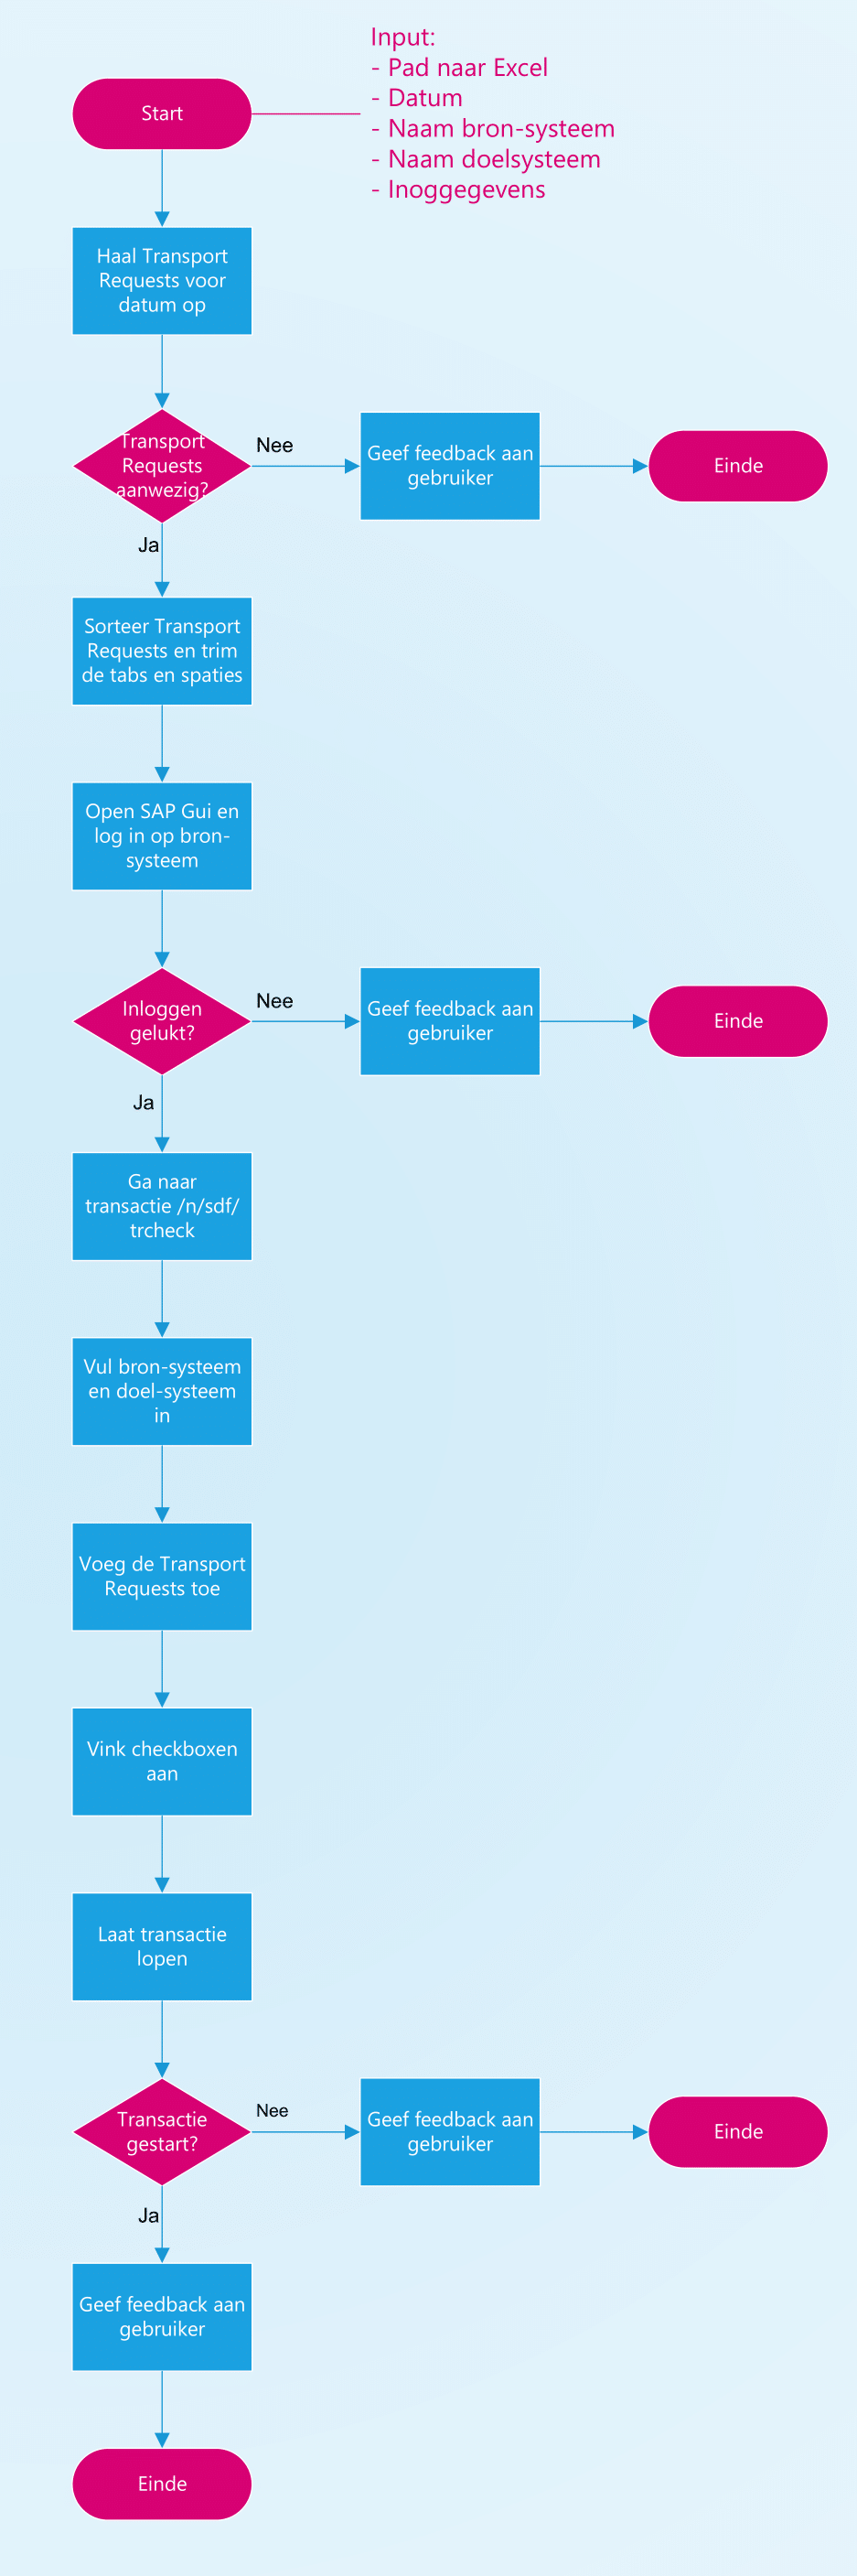
\includegraphics[width=0.5\textwidth]{../pictures/Flow_Cropped.png}
    \caption{Flow van het proces}
    \label{fig:flowchart}
\end{figure}
\label{fig:flowchart}

\subsection{Ontwikkeling van de Proof of Concept}
\label{subsec:ontwikkeling-proof-of-concept}

Het aanmaken van een RPA-automatisering via SAP BPA gebeurt in de BPA lobby. Op deze pagina worden alle eerder gecreëerde automatiseringen binnen het bedrijf getoond. Van hieruit wordt een nieuwe automatisering gecreëerd, waarna deze kan ontwikkeld worden binnen de BPA Process Editor. De process editor is de ontwikkelingsomgeving van SAP BPA.
Deze editor lijkt sterk op een flowchart-editor, wat logisch is als het seriële karakter van automatiseringsstappen bekeken wordt. De verschillende stappen worden één voor één gecreëerd en aan elkaar gelinkt. Hierbij kunnen variabelen worden doorgegeven en kunnen er verschillende condities zoals if-else-statements en loops geïmplementeerd worden.
Hieronder bespreken we kort de gecreëerde automatisering met de verschillende stappen.

\subsubsection{Start-formulier}
\label{subsubsec:start-formulier}

Zoals in de flowchart, die uit de design fase is ontstaan te zien is, heeft de automatisering verschillende input parameters nodig om de voorgestelde taken uit te kunnen voeren. Via de form te zien op afbeelding \ref{fig:startup-formulier} kunnen deze door de gebruiker opgegeven worden en kunnen deze gebruikt worden binnen de automatisering.
De verschillende waardes die opgegeven moeten worden zijn:

\begin{itemize}
    \item ExcelPad: het relatieve pad op het systeem van de gebruiker waar het Excel-bestand met de Transport Requests zich bevindt.
    \item Datum: de datum waarop de Transport Requests gefilterd moeten worden.
    \item BronSysteem: de naam van het systeem vanwaar de Transport Requests komen.
    \item DoelSysteem: de naam van het systeem naar waar de Transport Requests moeten overgezet worden.
    \item Gebruikersnaam: de gebruikersnaam van de gebruiker.
    \item Wachtwoord: het wachtwoord van de gebruiker.
    \item SysteemNaam: de connectie-naam waaronder het SAP-systeem is opgeslaan.
\end{itemize}

\begin{figure}
    \centering
    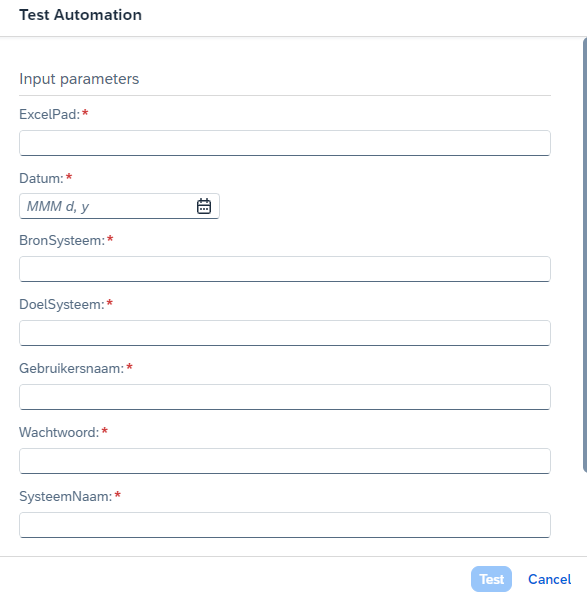
\includegraphics[width=0.8\textwidth]{../pictures/Startup_Form.png}
    \caption{Het start-formulier van de automatisering}
    \label{fig:startup-formulier}
\end{figure}

\subsubsection{Uitlezen van het Excel-bestand}
\label{subsubsec:uitlezen-excel}

De eerste grote stap die ondernomen wordt binnen de automatisering is het uitlezen van de Transport Requests uit het Excel-bestand. Hiervoor wordt het pad die de gebruiker bij de start heeft opgegeven, gebruikt om het Excel bestand te openen. Hierna kijkt de automatisering hoeveel lijnen het bestand kent, en via deze informatie haalt het alle informatie omtrent de Transport Requests uit het Excel-bestand via de Excel Cloud Link data-extractie taak.
Deze stappen zijn te zien op afbeelding \ref{fig:excel-lezen}.

\begin{figure}
    \centering
    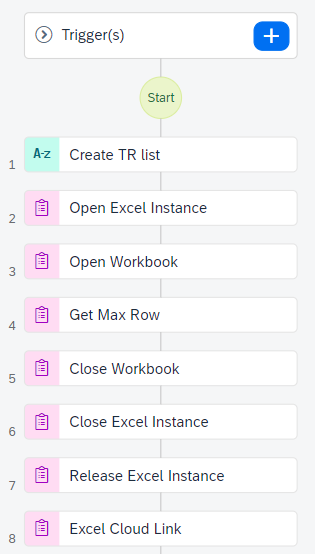
\includegraphics[width=0.8\textwidth]{../pictures/Read_Excel.png}
    \caption{Uitlezen van het Excel-bestand}
    \label{fig:excel-lezen}
\end{figure}

\subsubsection{Filteren van de Transport Requests}
\label{subsubsec:filteren-transport-requests}

Niet alle Transport Requests die in het Excel-bestand zijn opgeslagen moeten op hetzelfde moment overgezet worden. Via de datum die de gebruiker meegegeven heeft bij de start, worden de Transport Requests gefilterd. Enkel degene die op de opgegeven datum overgezet moeten worden worden aan de interne Transport Request lijst toegevoegd voor verdere verwerking.
Wanneer de Transport Requests gefilterd zijn en de te verwerken lijst is leeg, stopt de automatisering en wordt een melding gegeven aan de gebruiker.
Deze stappen zijn te zien op afbeelding \ref{fig:filter-transport-requests}.

\begin{figure}
    \centering
    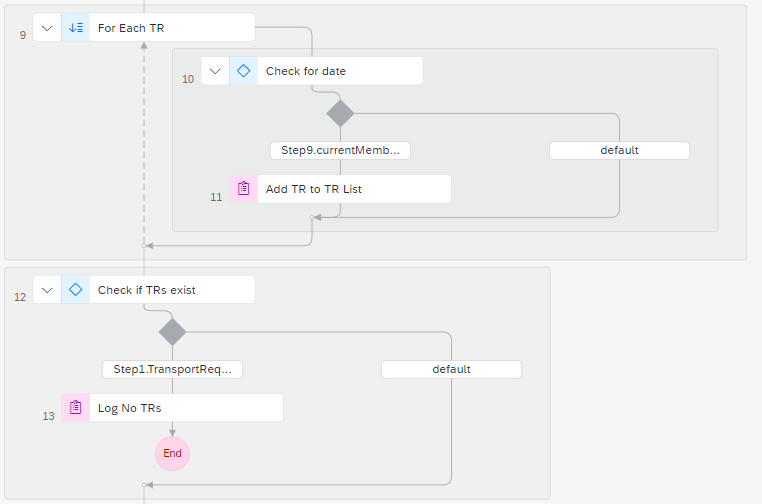
\includegraphics[width=0.8\textwidth]{../pictures/Check_Valable_TRs.png}
    \caption{Filteren van de Transport Requests}
    \label{fig:filter-transport-requests}
\end{figure}

\subsubsection{Inloggen bij SAP GUI}
\label{subsubsec:inloggen-sap-gui}

Nu de Transport Requests die gecontroleerd moeten worden gekend zijn, is het tijd voor de automatisering om zich in te loggen in de SAP GUI applicatie. Dit gebeurt in twee stappen. Eerst wordt de SAP GUI applicatie geopend en worden alle opgeslagen connecties opgehaald. De waardes van deze lijst worden dan één voor één vergeleken met de naam van het systeem die de gebruiker heeft meegegeven bij de start. Wanneer een connectie gevonden wordt die gelijk is aan deze meegegeven naam, wordt de positie in de lijst hiervan opgeslaan.
Deze stappen zijn te zien op afbeelding \ref{fig:controleren-connection-string}.

\begin{figure}
    \centering
    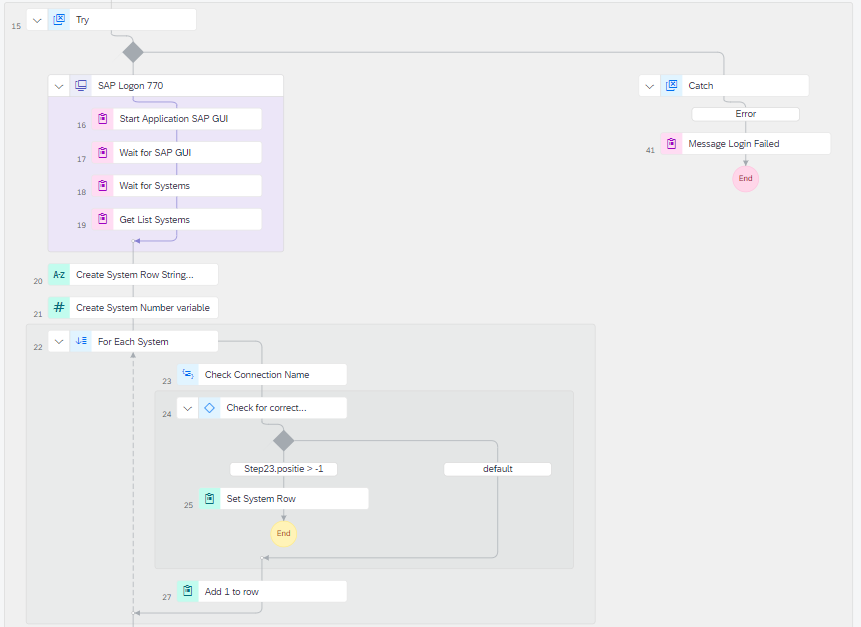
\includegraphics[width=0.8\textwidth]{../pictures/Check_Connection_String.png}
    \caption{Controleren van verschillende connecies}
    \label{fig:controleren-connection-string}
\end{figure}

Hierna wordt eerst gekeken of de connectie wel degelijk gevonden is. Wanneer dit niet het geval is wordt een melding getoond aan de gebruiker en stopt de automatisering.
Wanneer de connectie wel gevonden is, wordt deze via de berekende positie geopend en worden de inloggegevens van de gebruiker gebruikt om in te loggen binnen het systeem.
Deze stappen zijn te zien op afbeelding \ref{fig:inloggen-sap-gui}.

\begin{figure}
    \centering
    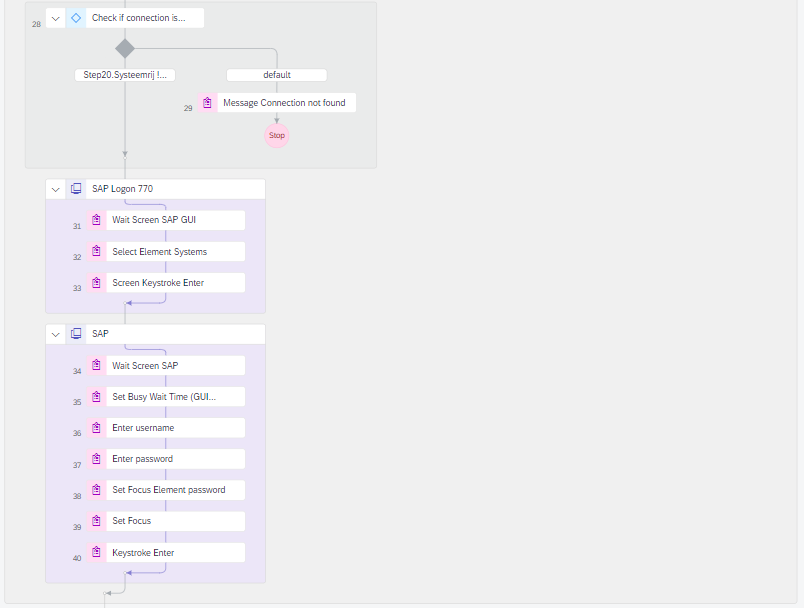
\includegraphics[width=0.8\textwidth]{../pictures/Login.png}
    \caption{Inloggen binnen SAP GUI}
    \label{fig:inloggen-sap-gui}
\end{figure}

Het volledige inlogproces staat binnen een try-catch block. Wanneer een stap zou falen, wordt er een bericht getoond aan de gebruiker en stopt de automatisering.

\subsubsection{Invullen van de de checken gegevens}
\label{subsubsec:invullen-checken-gegevens}

Nu de automatisering ingelogd is binnen het systeem kan de transactie om de Transport Requests te controleren geopend worden.
Wanneer deze geopend is worden zowel het bron-systeem als het doel-systeem ingevuld met de gegevens die de gebruiker bij de start van de automatisering heeft meegegeven.
Deze stappen zijn te zien op afbeelding \ref{fig:invullen-systemen}.

\begin{figure}
    \centering
    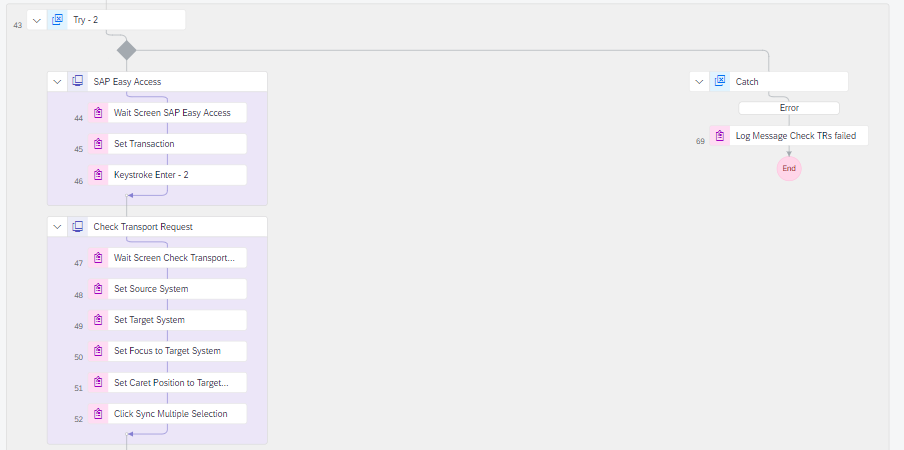
\includegraphics[width=0.8\textwidth]{../pictures/Set_Source_And_Target_System.png}
    \caption{Invullen van de systemen}
    \label{fig:invullen-systemen}
\end{figure}

Hierna wordt de lijst met gefilterde Transport Requests overlopen en worden ze ingevuld in de daartoe bestemde GUI tabel. Wanneer de volledige lijst ingevoegd is checkt de automatisering of de Transport Requests op een goede manier ingevuld zijn.
Deze stappen zijn te zien op afbeelding \ref{fig:controleren-transport-requests}.

\begin{figure}
    \centering
    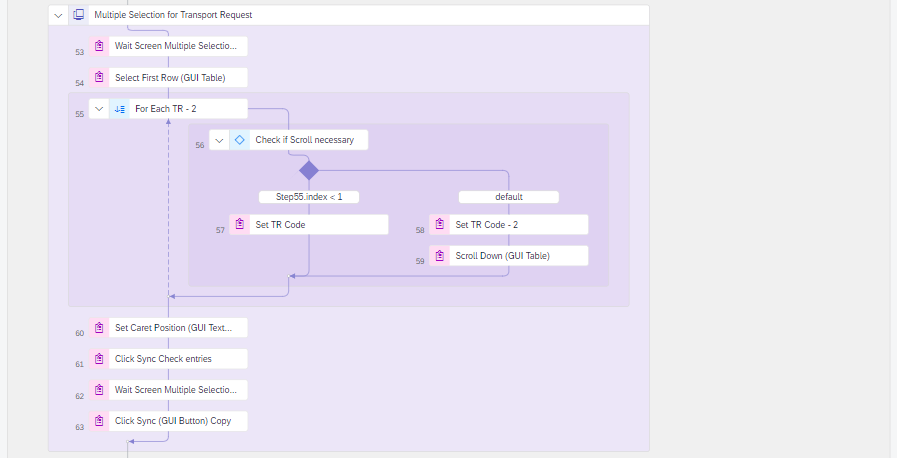
\includegraphics[width=0.8\textwidth]{../pictures/Enter_TRs.png}
    \caption{Invullen van de Transport Requests}
    \label{fig:controleren-transport-requests}
\end{figure}

Ook dit deel staat volledig binnen een try-catch block, dus wanneer de automatisering faalt wordt een melding getoond aan de gebruiker en stopt de automatisering.

\subsubsection{Controleren van de Transport Requests}
\label{subsubsec:controleren-transport-requests}

Nu alle gegevens ingevuld zijn vinkt de automatisering de checkboxes 'Cross Reference' en 'Sequence Check', de twee zaken die de automatisering moet controleren, aan. Hierna wordt de check gestart en geeft de automatisering het systeem terug aan de gebruiker. Wanneer de check voltooid is worden de resultaten van de check getoond en kan de gebruiker aan de slag met deze informatie.
Deze laatste stappen zijn te zien op afbeelding \ref{fig:controleren-trs}.

\begin{figure}
    \centering
    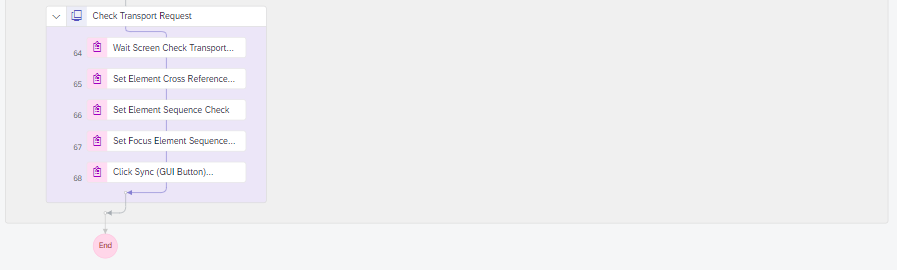
\includegraphics[width=0.8\textwidth]{../pictures/Checks.png}
    \caption{Controleren van de Transport Requests}
    \label{fig:controleren-trs}
\end{figure}

\subsection{Testen van de Proof of Concept}
\label{subsec:testen-proof-of-concept}

Wanneer de automatisering ontwikeld is, is het natuurlijk zeer belangrijk om deze te testen. Delaware heeft, als SAP-verdeler, een eigen testomgeving waarin mock-data beschikbaar is die een echt SAP-systeem nabootst. Dit is een uitgelezen manier om de automatisering te testen.
De automatisering werd een paar keer uitgevoerd en van dichtbij gemonitord om te zien of alle stappen wel degelijk op een goeie manier doorlopen werden. Ook werd het eindresultaat bekeken en getoetst aan de verwachtingen. De bot werd ook uitgevoerd met incorrecte gegevens, om te zien of het kan omgaan met uitzonderingen en deze op een correcte manier opvangt en rapporteert naar de gebruiker.

\section{Vergelijking met de huidige manier van werken}
\label{sec:vergelijking-huidige-manier}

Nu de Proof of Concept volledig uitgewerkt is, is het belangrijk om deze te vergelijken met de huidige manier van werken. Dit wordt op twee verschillende manieren gedaan. Als eerste wordt er gekeken naar de mogelijke tijdswinst die de automatisering oplevert.
Als tweede werd de consultant ondergevraagd over zijn mening over het gebruik van de automatisering. Hierbij wordt er gepolst naar of de automatisering het juiste proces uitvoert, de performantie en of het in zijn mening zijn werk zal vergemakkelijken.

\subsection{Tijdswinst}
\label{subsec:tijdswinst}

Om de tijdswinst van de automatisering te berekenen werd het proces 2 keer uitgevoerd door de betrokken consultant. De eerste keer werd het manueel uitgevoerd, zoals het nu dagelijks gebeurd. De tweede keer wordt de automatisering uit de Proof of Concept gebruikt.
Beide uitvoeringen werden getimed en de resultaten werden in tabel \ref{tab:tijdswinst} vergeleken.

\begin{table}[h]
    \centering
        \begin{tabular}{|l|l|}
            \hline
            & Tijd \\ \hline
            Manueel & 125,55 seconden \\ \hline
            RPA-automatisering & 24,39 seconden \\ \hline
            Tijdswinst & 101,16 seconden \\ \hline
        \end{tabular}
    \caption{Vergelijking van de duur van het proces met en zonder automatisering}
    \label{tab:tijdswinst}
\end{table}

Uit deze resultaten kan duidelijk afgeleid worden dat het proces duidelijk sneller uitgevoerd wordt via de automatisering. De automatisering werkt 5 keer sneller dan wanneer het manueel wordt uitgevoerd.
Wanneer dit proces dagelijks wordt uitgevoerd, kan deze automatisering over een lange tijdsperiode een zeer grote tijdswinst opleveren voor de consultant.

\subsection{Gebruiksgemak}
\label{subsec:gebruiksgemak}

Naast de tijdswinst is het voor nieuwe technologieën ook belangrijk dat de toekomstige gebruikers ook overtuigd zijn van de mogelijkheden ervan. Daarom werd de consultant, nadat hij de automatisering gebruikt had, ondervraagd naar zijn menig hierover.
Op de vraag of de automatisering het juiste proces uitvoert en het dit op een correcte manier uitvoert, antwoordde de consultant dat dit zeker het geval is. Ook merkte hij zelf op dat de automatisering in bijna elke stap sneller werkt dan hij de stap zou kunnen uitvoeren.
Op de vraag of hij de automatisering zou vertrouwen om deze taak uit te voeren, antwoordde hij dat dit niet direct het geval zou zijn. Zoals elke nieuwe tool zou hij de eerste dagen toch het resultaat een controleren en kijken of elk Transport Request wel degelijk meegegeven werd. Maar hij is ervan overtuigd dat er na een paar dagen zeker meer vertrouwen zal zijn in de automatisering en dat deze controle achterwege zal kunnen gelaten worden.
Op de laatste vraag, of hij denkt dat de automatisering zijn dagelijkse werk zal vergemakkelijken, antwoordde hij duidelijk ja. Hij gaf zelf aan dat, alhoewel het een vrij kort proces is, hij hier toch dagelijks tijd mee verliest en dit soms zeer frustrerend kan zijn, en deze automatisering hier een zeer grote hulp voor kan bieden.

Uit de antwoorden van de consultant kan duidelijk afgeleid worden dat hij zeer positief reageerde tegenover de automatisering en dat hij deze in de toekomst zeker zou gebruiken.
%%=============================================================================
%% Conclusie
%%=============================================================================

\chapter{Conclusie}%
\label{ch:conclusie}

% TODO: Trek een duidelijke conclusie, in de vorm van een antwoord op de
% onderzoeksvra(a)g(en). Wat was jouw bijdrage aan het onderzoeksdomein en
% hoe biedt dit meerwaarde aan het vakgebied/doelgroep? 
% Reflecteer kritisch over het resultaat. In Engelse teksten wordt deze sectie
% ``Discussion'' genoemd. Had je deze uitkomst verwacht? Zijn er zaken die nog
% niet duidelijk zijn?
% Heeft het onderzoek geleid tot nieuwe vragen die uitnodigen tot verder 
%onderzoek?

\lipsum[76-80]



%---------- Bijlagen -----------------------------------------------------------

\appendix

\chapter{Onderzoeksvoorstel}

Het onderwerp van deze bachelorproef is gebaseerd op een onderzoeksvoorstel dat vooraf werd beoordeeld door de promotor. Dat voorstel is opgenomen in deze bijlage.

%% TODO: 
\section*{Samenvatting}
\begin{abstract}
    Tijdens de klantenservice van een project heeft een consultant verschillende gegevens nodig om de klant op een goede manier te helpen. Het opzoeken van deze gegevens kan soms de nodige tijd nemen, wat frustrerend is voor zowel de consultant als de klant. Deze bachelorproef zal kijken naar de mogelijkheid om Robotic Process Automation te gebruiken om de betrokken consultant te helpen met verschillende kleinere taken binnen de klantenservice, zoals bij het opzoeken van nodige informatie. Dit kan de ervaring voor zowel de consultant als de klant verbeteren. Er zullen verschillende processen onderzocht worden die voorkomen tijdens de klantenservice. Deze processen zal ik halen uit een interview met een betrokken consultant. De gevonden processen zullen vergeleken worden en hieruit zal dan 1 proces gekozen worden die uitgewerkt zal worden als een Proof of Concept. Voor de Proof of Concept zal ik ook eerst een vergelijking maken tussen verschillende RPA-verdelers en hieruit de meest geschikte keuze maken. Het verwachte resultaat zal enerzijds een lijst met verschillende processen zijn waar een automatisering kan voor worden opgezet, en anderzijds een uitgewerkte automatisering die gebruikt kan worden door de betrokken Consultants. Als conslusie verwacht ik veel kleine processen te vinden die geautomatiseerd kunnen worden via Robotic Process Automation. Wanneer deze dan geautomatiseerd zijn verwacht ik zeker een bepaalde tijdwinst, maar vooral een betere ervaring voor de betrokken consultants. Deze kunnen zich nu meer focussen op de klant en minder op het opzoeken van informatie.
\end{abstract}

%---------- Inleiding ---------------------------------------------------------

\section{Introductie}%
\label{sec:introductie}

% Waarover zal je bachelorproef gaan? Introduceer het thema en zorg dat volgende zaken zeker duidelijk aanwezig zijn:

% \begin{itemize}
%   \item kaderen thema
%   \item de doelgroep
%   \item de probleemstelling en (centrale) onderzoeksvraag
%   \item de onderzoeksdoelstelling
% \end{itemize}

% Denk er aan: een typische bachelorproef is \textit{toegepast onderzoek}, wat betekent dat je start vanuit een concrete probleemsituatie in bedrijfscontext, een \textbf{casus}. Het is belangrijk om je onderwerp goed af te bakenen: je gaat voor die \textit{ene specifieke probleemsituatie} op zoek naar een goede oplossing, op basis van de huidige kennis in het vakgebied.

% De doelgroep moet ook concreet en duidelijk zijn, dus geen algemene of vaag gedefinieerde groepen zoals \emph{bedrijven}, \emph{developers}, \emph{Vlamingen}, enz. Je richt je in elk geval op it-professionals, een bachelorproef is geen populariserende tekst. Eén specifiek bedrijf (die te maken hebben met een concrete probleemsituatie) is dus beter dan \emph{bedrijven} in het algemeen.

% Formuleer duidelijk de onderzoeksvraag! De begeleiders lezen nog steeds te veel voorstellen waarin we geen onderzoeksvraag terugvinden.

% Schrijf ook iets over de doelstelling. Wat zie je als het concrete eindresultaat van je onderzoek, naast de uitgeschreven scriptie? Is het een proof-of-concept, een rapport met aanbevelingen, \ldots Met welk eindresultaat kan je je bachelorproef als een succes beschouwen?
Klantenservice kent veel kleine, repetitieve taken die tijd in beslag nemen zowel voor de werknemer, als voor de klant. Hierbij kan gedacht worden aan het ophalen van de juiste klantengegevens, de gegevens van collega's op het project of voorbije pogingen om het probleem op te lossen. 

Deze bachelorproef wil onderzoeken of het mogelijk is om via Robotic Process Automation deze taken te automatiseren, zodat de werknemer meer bezig kan zijn met de echte problemen van de klant, en deze dus een betere en snellere klantenservice ontvangt.

De doelgroep van deze bachelorproef zijn de SAP consultants van het bedrijf delaware. Deze werknemers komen dagelijks in contact met klanten, maar aangezien ze als consultants vaak met meerdere klanten werken, kunnen de gegevens van deze klanten soms verward geraken.

De centrale onderzoeksvraag van deze bachelorproef is waar en hoe makkelijk Robotic Process Automation kan ingezet worden tijdens de klantenservice. Concreet heeft deze vraag twee deelvragen: 

\begin{itemize}
  \item Welke taken kan Robotic Process Automation automatiseren?
  \item Welke meerwaarde hebben deze automatiseringen? Hierbij denken we aan tijdwinst en gebruiksgemak voor de consultant.
\end{itemize}

De doelstelling van deze bachelorproef is tweeledig. Als eerste zal uitgezocht worden voor welke taken Robotic Process Automation een verbetering kan zijn. Ten tweede zal er ook een Proof of Concept Automation aangemaakt worden voor een van deze taken die makkelijk bruikbaar is voor de consultants van delaware. Hiervoor zal ook bekeken worden of het beter is de technologiën die delaware al heeft te gebruiken (SAP Build Process Automation, UIPath), of er beter gekeken wordt naar andere technologiën, zoals Automation Anywhere en Blue Prism. 

Het al dan niet slagen van deze proof of concept zal op 3 verschillende criteria bekeken worden:
\begin{itemize}
  \item Voor de start zal er aan een consultant gevraagd worden wat hij of zij verwacht van het resultaat. De uitgewerkte proof of concept zal dan vergeleken worden met deze vooropgestelde verwachtingen.
  \item Er zal een kleine test uitgevoerd worden waarin een consultant verschillende kleine taken moet uitvoeren met en zonder de uitgewerkte proof of concept. Hieruit zal de eventuele tijdswinst gemeten kunnen worden.
  \item Nadat consultants de proof of concept gebruikt hebben zal er gevraagd worden naar hun ervaringen met de proof of concept. Hieruit kan het gebruiksgemak afgeleid worden.
\end{itemize}
Uit deze 3 criteria kan dan een finaal oordeel worden gemaakt omtrent de onderzoeksvraag.

%---------- Stand van zaken ---------------------------------------------------

\section{State-of-the-art}%
\label{sec:state-of-the-art}

\subsection{Wat is Robotic Process Automation}
\label{Wat is Robotic Process Automation}
Robotic Process Automation is een manier van processen automatiseren die gebruik maakt van de presentatielaag van applicaties. Hierdoor kan het vergeleken worden met oudere ‘screen-scraping’ concepten. Het grote verschil is dat RPA ook gebruik maakt van machine learning en definiëren van UI-elementen zodat de verkregen automation robuuster is dan zijn voorgangers. 
Als de lay-out van een pagina wordt aangepast, leert RPA hiermee om te gaan, net zoals een menselijke actor. Hierdoor is het mogelijk om betrouwbaar informatie af te lezen van een scherm en deze in andere applicaties te gebruiken. Deze vorm van ontwikkelen is vaak sneller dan een volledige applicatie te ontwikkelen, waardoor Robotic Process Automation hiervoor een goedkoper alternatief kan zijn. RPA opent zo de mogelijkheid om repetitieve taken te automatiseren en meer tijd vrij te maken voor de werknemers om meer humane en interessantere taken uit te voeren \autocite{Panikkar2022}.

\subsection{Unattended en Attended bots}
\label{Unattended en Attended bots}
Er bestaan twee verschillende soorten RPA-bots. Attended bots zijn automations die gebruikt worden om een menselijke gebruiker te assisteren. 
Unattended bots kunnen gestart worden door een trigger en hebben geen interactie meer nodig op hun process tot een goed einde te brengen. Door het bekijken van de complexiteit van een process kan beslist worden voor een van deze concepten want ze hebben beiden hun voordelen en nadelen.

\subsection{Waarom RPA}
\label{Waarom RPA}
Elk bedrijf heeft veel taken die er baat van zouden hebben geautomatiseerd te worden. Dit kan zorgen voor tijdwinst, maar ook een verbetering in de tevredenheid van de werknemers. Volgens \textcite{blueprism2023} zou bijvoorbeeld 88 procent van de bedrijfsleiders zich gelukkiger voelen als ze zich dankzij automatisering minder op administratief werk hoefden te concentreren. RPA is een eenvoudige en snelle oplossingen om de zeer herhaaldelijke en dus dure taken makkelijk te automatiseren. Hierdoor kunnen bedrijven revalueren welke taken wel geautomatiseerd worden en welke niet. Het feit dat in 2021 al bijna 20 procent van de bedrijven gebruikt maakt van RPA in een bepaalde zin \autocite{CemDilmegani2023}, toon aan hoe belangrijk deze technologie kan worden in de toekomst.

\subsection{RPA-verdelers}
\label{RPA-verdelers}
RPA is een vrij nieuwe tool met veel mogelijkheden, dus er is een grote markt aan RPA-verdelers. Deze zijn onder andere:

\begin{itemize}
  \item SAP Build Process Automation
  \item UIPath
  \item Blue Prism
  \item Automation Anywhere
\end{itemize}

Sommige van deze verdelers zijn vooral gericht op een specifiek systeem, zoals SAP Build Process Automation die vooral op SAP-producten gefocust is. Anderen zijn meer algemeen. Door de sterktes, zwaktes en visies van deze verkopers te bekijken kan ik ook een beter idee vormen van de RPA-oplossingen

\subsection{Veiligheid}
\label{Veiligheid}
Het fout automatiseren van taken en zo foute output produceren kan zowel werknemer als klant frustreren, dus wordt er ook onderzocht of men makkelijk een automation kan testen op foute output en deze oplossen.


% Hier beschrijf je de \emph{state-of-the-art} rondom je gekozen onderzoeksdomein, d.w.z.\ een inleidende, doorlopende tekst over het onderzoeksdomein van je bachelorproef. Je steunt daarbij heel sterk op de professionele \emph{vakliteratuur}, en niet zozeer op populariserende teksten voor een breed publiek. Wat is de huidige stand van zaken in dit domein, en wat zijn nog eventuele open vragen (die misschien de aanleiding waren tot je onderzoeksvraag!)?

% Je mag de titel van deze sectie ook aanpassen (literatuurstudie, stand van zaken, enz.). Zijn er al gelijkaardige onderzoeken gevoerd? Wat concluderen ze? Wat is het verschil met jouw onderzoek?

% Verwijs bij elke introductie van een term of bewering over het domein naar de vakliteratuur, bijvoorbeeld~\autocite{Hykes2013}! Denk zeker goed na welke werken je refereert en waarom.

% Draag zorg voor correcte literatuurverwijzingen! Een bronvermelding hoort thuis \emph{binnen} de zin waar je je op die bron baseert, dus niet er buiten! Maak meteen een verwijzing als je gebruik maakt van een bron. Doe dit dus \emph{niet} aan het einde van een lange paragraaf. Baseer nooit teveel aansluitende tekst op eenzelfde bron.

% Als je informatie over bronnen verzamelt in JabRef, zorg er dan voor dat alle nodige info aanwezig is om de bron terug te vinden (zoals uitvoerig besproken in de lessen Research Methods).

% % Voor literatuurverwijzingen zijn er twee belangrijke commando's:
% % \autocite{KEY} => (Auteur, jaartal) Gebruik dit als de naam van de auteur
% %   geen onderdeel is van de zin.
% % \textcite{KEY} => Auteur (jaartal)  Gebruik dit als de auteursnaam wel een
% %   functie heeft in de zin (bv. ``Uit onderzoek door Doll & Hill (1954) bleek
% %   ...'')

% Je mag deze sectie nog verder onderverdelen in subsecties als dit de structuur van de tekst kan verduidelijken.

%---------- Methodologie ------------------------------------------------------
\section{Methodologie}%
\label{sec:methodologie}
Dit onderzoek zal bestaan uit 3 grote fases.
\subsection{Fase 1: Interviews met Consultants}
\label{Fase 1: Interviews met Consultants}
In de eerste fase zullen er interviews met verschillende consultants uitgevoerd worden. Uit deze interviews zal afgeleid worden welke taken repetitief zijn en veel tijd in beslag nemen. Deze taken zullen dan opgelijst worden. Uit deze lijst zal ik dan kijken hoe makkelijk bepaalde taken geautomatiseerd kunnen worden en hoeveel tijd de Consultant hier mee zou kunnen winnen.
Deze fase zal 3 weken in beslag nemen.
\subsection{Fase 2: Literatuurstudie}
\label{Fase 2: Literatuurstudie}
In deze fase van de bachelorproef zal er een literatuurstudie uitgevoerd worden. In deze studie zal ik allereerst de mogelijkheden van Robotic Process Automation onderzoeken. Hiernaast zal ik ook de de verschillende Robotic Process Automation verdelers vergelijken en de positieve en negatieve punten oplijsten per verdeler.
Deze fase zal 4 weken in beslag nemen.
\subsection{Fase 3: Beslissing en Proof of Concept}
\label{Fase 3: Beslissing en Proof of Concept}
In de laatste fase van deze bachelorproef zal een process gekozen worden om te automatiseren. Ik zal ook een bepaalde RPA-verdeler kiezen en dus met deze technologie de automatisering uitwerken.
Deze fase zal 4 weken in beslag nemen.

% Hier beschrijf je hoe je van plan bent het onderzoek te voeren. Welke onderzoekstechniek ga je toepassen om elk van je onderzoeksvragen te beantwoorden? Gebruik je hiervoor literatuurstudie, interviews met belanghebbenden (bv.~voor requirements-analyse), experimenten, simulaties, vergelijkende studie, risico-analyse, PoC, \ldots?

% Valt je onderwerp onder één van de typische soorten bachelorproeven die besproken zijn in de lessen Research Methods (bv.\ vergelijkende studie of risico-analyse)? Zorg er dan ook voor dat we duidelijk de verschillende stappen terug vinden die we verwachten in dit soort onderzoek!

% Vermijd onderzoekstechnieken die geen objectieve, meetbare resultaten kunnen opleveren. Enquêtes, bijvoorbeeld, zijn voor een bachelorproef informatica meestal \textbf{niet geschikt}. De antwoorden zijn eerder meningen dan feiten en in de praktijk blijkt het ook bijzonder moeilijk om voldoende respondenten te vinden. Studenten die een enquête willen voeren, hebben meestal ook geen goede definitie van de populatie, waardoor ook niet kan aangetoond worden dat eventuele resultaten representatief zijn.

% Uit dit onderdeel moet duidelijk naar voor komen dat je bachelorproef ook technisch voldoen\-de diepgang zal bevatten. Het zou niet kloppen als een bachelorproef informatica ook door bv.\ een student marketing zou kunnen uitgevoerd worden.

% Je beschrijft ook al welke tools (hardware, software, diensten, \ldots) je denkt hiervoor te gebruiken of te ontwikkelen.

% Probeer ook een tijdschatting te maken. Hoe lang zal je met elke fase van je onderzoek bezig zijn en wat zijn de concrete \emph{deliverables} in elke fase?

%---------- Verwachte resultaten ----------------------------------------------
\section{Verwacht resultaat, conclusie}%
\label{sec:verwachte_resultaten}
\subsection{Verwacht resultaat}
\label{Verwacht resultaat}
Er wordt verwacht dat er in het klantenservice process verschillende repetitieve kleine taken zijn die gemakkelijk te automatiseren zijn. Hieruit zal dan een automatisering gekozen worden die veel impact zou kunnen hebben op de snelheid van dienstverlening. Deze automatisering zal dan uitgewerkt worden, en in het ideale scenario gebruikt worden door de consultants van delaware.
\subsection{Verwachte conclusie}
\label{Verwachte conclusie} 
Robotic Process Automation zal waarschijnlijk niet alle repetitieve taken van menselijke werknemers overnemen, maar kan de klantervaring op een zeer efficiënte manier verbeteren. Dit doordat de consultant zich minder hoeft bezig te houden met het opzoeken van informatie, en zich hierdoor dus meer kan bezighouden met het effectief helpen van de klant. Het is een goedkope, snelle manier van automatiseren met een grote return of investment. De tool zelf staat ook nog in zijn kinderschoenen waardoor verwacht wordt dat de mogelijkheden van de tool nog zullen verbeteren.  


% Hier beschrijf je welke resultaten je verwacht. Als je metingen en simulaties uitvoert, kan je hier al mock-ups maken van de grafieken samen met de verwachte conclusies. Benoem zeker al je assen en de onderdelen van de grafiek die je gaat gebruiken. Dit zorgt ervoor dat je concreet weet welk soort data je moet verzamelen en hoe je die moet meten.

% Wat heeft de doelgroep van je onderzoek aan het resultaat? Op welke manier zorgt jouw bachelorproef voor een meerwaarde?

% Hier beschrijf je wat je verwacht uit je onderzoek, met de motivatie waarom. Het is \textbf{niet} erg indien uit je onderzoek andere resultaten en conclusies vloeien dan dat je hier beschrijft: het is dan juist interessant om te onderzoeken waarom jouw hypothesen niet overeenkomen met de resultaten.



%%---------- Andere bijlagen --------------------------------------------------
% TODO: Voeg hier eventuele andere bijlagen toe. Bv. als je deze BP voor de
% tweede keer indient, een overzicht van de verbeteringen t.o.v. het origineel.
%\input{...}
%%---------- Backmatter, referentielijst ---------------------------------------

\backmatter{}

\setlength\bibitemsep{2pt} %% Add Some space between the bibliograpy entries
\printbibliography[heading=bibintoc]

\end{document}
